%%%%%%%%%%%%%%%%%%%%%%% preamble %%%%%%%%%%%%%%%%%%%%%%%%%%%
\documentclass[10pt,letterpaper]{article}
\usepackage{opex3}
\usepackage{epstopdf}
\usepackage{color}
\usepackage{amsmath}
\usepackage{amssymb}
\usepackage{graphicx}
\usepackage{multirow}
\usepackage{caption}
\usepackage{subcaption}
\usepackage{floatrow}
\newfloatcommand{capbtabbox}{table}[][\FBwidth]
\usepackage{blindtext}
\usepackage{cite}
\usepackage{array}


\makeatletter
\newcommand*{\rmnum}[1]{\expandafter\@slowromancap\romannumeral #1@}
\makeatother
\newcommand{\vm}[1]{{\bf{#1}}}
\newcommand{\vecttwo}[2]
{
	\left[
		\begin{eqnarray*}
		#1\\
		#2
		\end{eqnarray*}
	\right]
}
\newcommand{\vectthree}[3]
{
	\left[
		\begin{eqnarray*}
		#1\\
		#2\\
		#3
		\end{eqnarray*}
	\right]
}

%%%%%%%%%%%%%%%%%%%%%%% begin %%%%%%%%%%%%%%%%%%%%%%%%%%%%%%
\begin{document}

%%%%%%%%%%%%%%%%%% title page information %%%%%%%%%%%%%%%%%%
\title{Impact of visual perception on the performance of Color Shift Keying modulation in IEEE 802.15.7}

\author{Pankil M. Butala$^{1,2}$, Hany Elgala$^{1,3}$ and Thomas D.C. Little$^{1,4}$}

\address{$^{1}$Multimedia Communication Laboratory and Smart Lighting Engineering Research Center\\
Boston University, Boston, MA 02215, USA\\
\{$^2$pbutala,$^3$helgala,$^4$tdcl\}@bu.edu}

% \homepage{http:...} %% author's URL, if desired

%%%%%%%%%%%%%%%%%%% abstract and OCIS codes %%%%%%%%%%%%%%%%
%% [use \begin{abstract*}...\end{abstract*} if exempt from copyright]

\begin{abstract}
The IEEE 802.15.7 standard defines specifications for short-range optical wireless communication (OWC) using visible light. The standard specifies color shift keying (CSK) as the preferred modulation scheme for indoor OWC while simultaneously providing illumination. This article considers the performance of $M$-ary CSK under the linear system model as specified in the standard. In light of illumination requirements, human eye's optical perception introduces unique non-linearities in the CSK signaling chain. It is shown that these non-linearities introduce performance penalties of more than 15 dB, 10 dB, and 5 dB for $M$ = 4, 8, and 16 CSK respectively. A new metric called luminous-signal-to-noise ratio (LSNR) is also introduced to fairly compare performance of any two OWC signaling schemes operating at a user defined illumination intensity level and is used to compare performance of $M$-ary CSK implemented with different colored sources. At a target bit error rate of $\leq 10^{-3}$, simulation results indicate that clipping negative receiver output does not have an impact on $M$-ary CSK performance.
\end{abstract}

\ocis{(060.2605) Free-space optical communication, (060.4080) Modulation, (060.4510) Optical communications} 
% REPLACE WITH CORRECT OCIS CODES FOR YOUR ARTICLE, MINIMUM OF TWO; Avoid using the OCIS codes for “General” or “General science” whenever possible.

%%%%%%%%%%%%%%%%%%%%%%% References %%%%%%%%%%%%%%%%%%%%%%%%%
\begin{thebibliography}{99}
\bibitem{cis14a} ``{Cisco visual networking index: forecast and methodology, 2013-2018},'' (2014).
\bibitem{elg11a} H. Elgala, R. Mesleh and H. Haas, ``{Indoor optical wireless communication: potential and state-of-the-art},'' IEEE Comm Mag. {\bf 49}(9), 56--62 (2011).
\bibitem{gan13a} J. Gancarz, H. Elgala and T.D.C. Little, ``{Impact of lighting requirements on VLC systems},'' IEEE Comm Mag. {\bf 51}(12), 34--41 (2013).
\bibitem{rah15a} M. Rahaim and T.D.C. Little, ``{Towards Practical Integration of Dual-Use VLC within 5G Networks},'' to appear in IEEE Wireless Comm. (2015).
%\bibitem{gru08b} J. Grubor, S. Randel, K-D Langer and J.W. Walewski, ``{Broadband Information Broadcasting Using LED-Based Interior Lighting},'' J. Lightwave Tech. {\bf 26}(24), 3883--3892 (2008).
%\bibitem{min08a} H. Minh, D. O'Brien, G. Faulkner, L. Zeng, K. Lee, D. Jung and Y. Oh, ``{High-Speed Visible Light Communications Using Multiple-Resonant Equalization},'' IEEE Photon. Lett. {\bf 20}(14), 1243--1245 (2008).
\bibitem{arm09a} J. Armstrong ``{OFDM for Optical Communications},'' J. Lightwave Tech. {\bf 27}(3), 189-204 (2009).
\bibitem{but14b} P. Butala, H. Elgala and T.D.C. Little, ``{Sample indexed spatial orthogonal frequency division multiplexing},'' Chin. Opt. Lett. {\bf 12}(9), 090602 (2014)
\bibitem{cskxy} A. Yokoi, J. Son and T. Bae, ``{CSK constellation in all color band combinations},'' {https://mentor.ieee.org/802.15/dcn/11/15-11-0247-00-0007-csk-constellation-in-all-color-band-combinations.pdf} (2011).
\bibitem{but12a} P. Butala, J. Chau and T.D.C. Little, ``{Metameric modulation for diffuse visible light communications with constant ambient lighting},'' Intl. Workshop on Opt. Wireless Comm. (IWOW), 1-3 (2012).
\bibitem{ieee802.15.7} ``{IEEE Standard for Local and Metropolitan Area Networks--Part 15.7: Short-Range Wireless Optical Communication Using Visible Light},'' (2011).
\bibitem{raj12a} S. Rajagopal, R.D. Roberts and S-K Lim, ``{IEEE 802.15.7 visible light communication: modulation schemes and dimming support},'' IEEE Comm. Mag. {\bf 50}(3), 72-82 (2012).
\bibitem{sin13a} R. Singh, T. O'Farrell and J.P.R. David, ``{Performance evaluation of IEEE 802.15.7 CSK physical layer},'' Globecom Workshops, IEEE 1064-1069 (2013).

%\bibitem{gallo99} K. Gallo and G. Assanto, ``All-optical diode based on second-harmonic generation in an asymmetric waveguide,'' \josab {\bf 16}(2), 267--269 (1999).
%{\bf volume}(issue)

\end{thebibliography}

%%%%%%%%%%%%%%%%%%%%%  Introduction  %%%%%%%%%%%%%%%%%%%%%%%
\section{Introduction}\label{sINTR}

The proliferation of mobile devices including smartphones, tablets,
and laptop computers is driving the need for increased capacity in
wireless networks. Current forecasts \cite{cis14a} show that our
wireless infrastructure must continually improve to sustain this level
of growth. However, there remains an imbalance between the devices'
ability to consume data and the networks' ability to service their
demand. Traffic ``offloading'' has become the mitigation strategy
whereby wireless access technologies such as WiFi are exploited for their
localized capacity and links to wired infrastructure. However, these
radio frequency (RF) solutions share limited available spectrum and face both scale and
deployment challenges.  Light-based media, in contrast, offer new
spectrum opportunities and characteristics such as line-of-sight and
security. This is fueling recent research on how to achieve
light-based communication \cite{elg11a}. At the same time, advances in solid state
materials have yielded highly-efficient light emitting diodes (LED) that have upended the lighting industry. Lighting companies now compete to replace all
existing lighting with the new energy-efficient LED devices. Because
lighting is well positioned to support human activities, it is also
well positioned to serve as a highly localized wireless access vehicle by modulating the visible spectrum (380 nm -- 780 nm). This model is called the ``dual
use'' of lighting and communication.  In a practical implementation,
overhead luminaires provide light and data downlink as an offload
medium, being augmented by the availability of other media including
RF as part of a heterogeneous network \cite{gan13a,rah15a}. 

Visible light communication (VLC) uses intensity-modulation
direct-detection (IM/DD) for wireless data transfer. Different modulation schemes used in conjunction with IM/DD have been
proposed for use with VLC. Optical orthogonal frequency division
multiplexing (O-OFDM) schemes provide high spectral efficiency for a
single-input single-output (SISO) VLC channel \cite{arm09a}. To
achieve better spectral efficiency, multiple-input multiple-output
(MIMO) techniques exploiting dimensions of space and color have also
been documented \cite{but14b,cskxy,but12a}.

The IEEE standard for short-range optical wireless communication (OWC) using
visible light specifies color shift keying (CSK)
as the modulation technique of choice under the physical layer (PHY)
\rmnum{3} specifications \cite{ieee802.15.7}. For the rest of this article, the noun `standard' shall imply the IEEE 802.15.7 standard, specifically chapter 12 on PHY \rmnum{3} specifications as in reference \cite{ieee802.15.7}. The standard outlines linear system configurations with $M$-ary CSK to achieve up to 96 Mb/s data rate. Reference \cite{raj12a} provides an overview of modulation and dimming techniques specified within the standard while reference \cite{sin13a} studies select color bands for CSK.

This article studies $M$-ary CSK for all color band combinations as
outlined in the standard and then extends the study to include
practical implementation constraints: (a) non-linearity in visual perception introduces non-linearity in illumination to radiant flux transformations and vice versa and (b) user
defined target illumination intensity level. In the process, a new
metric -- luminous-signal-to-noise ratio (LSNR) is introduced to
compare performance of different signaling schemes at a target
illumination intensity level.

An overview of CSK modulation technique is provided in
Section \ref{sCSK}. The linear CSK model as described in the standard is then outlined in Section \ref{sCSKL}. CSK performance considerations in a practical scenario due presence of non-linearity introduced by color to radiant flux transformation is
considered in Section \ref{sCSKNL}. Section \ref{sCSKLSNR} introduces
LSNR and CSK performance considerations due to practical illumination
constraints. Section \ref{sCONC} concludes the article.

%%%%%%%%%%%%%%%%%%  Color Shift Keying  %%%%%%%%%%%%%%%%%%%%
\section{Color Shift Keying}\label{sCSK}
LED based luminaires are energy efficient and are thus being widely
adopted in indoor spaces to provide illumination. In order to
dynamically control the rendered illumination spectrum, luminaires
contain multiple elements of at least three colors of LEDs. Different
rendered spectra, or spectral power distributions (SPDs), can be
generated by mixing different ratios of radiant flux emitted from the
multiple LEDs comprising a luminaire. Each resulting SPD realizes
a different color mix to the human eye.

\renewcommand{\arraystretch}{1.05}
\begin{figure}[b]
\begin{floatrow}
		\capbtabbox{
			\begin{tabular}{|c|c|c|c|c|}
			\hline
			\multirow{2}{*}{\textbf{CB$_{u}$}} & \textbf{Band} & \textbf{Center} & \multirow{2}{*}{\textbf{x}} & \multirow{2}{*}{\textbf{y}}\\
			 & \textbf{(nm)} & \textbf{(nm)} & & \\
			\hline
			CB$_{0}$ & 380 - 478 & 429 & 0.169 & 0.007\\
			\hline
			CB$_{1}$ & 478 - 540 & 509 & 0.011 & 0.733\\
			\hline
			CB$_{2}$ & 540 - 588 & 564 & 0.402 & 0.597\\
			\hline
			CB$_{3}$ & 588 - 633 & 611 & 0.669 & 0.331\\
			\hline
			CB$_{4}$ & 633 - 679 & 656 & 0.729 & 0.271\\
			\hline
			CB$_{5}$ & 679 - 726 & 703 & 0.734 & 0.265\\
			\hline
			CB$_{6}$ & 726 - 780 & 753 & 0.734 & 0.265\\
			\hline
			\multicolumn{5}{c}{ }
			\end{tabular}}
			{\caption{Color bands.}}
			\ffigbox{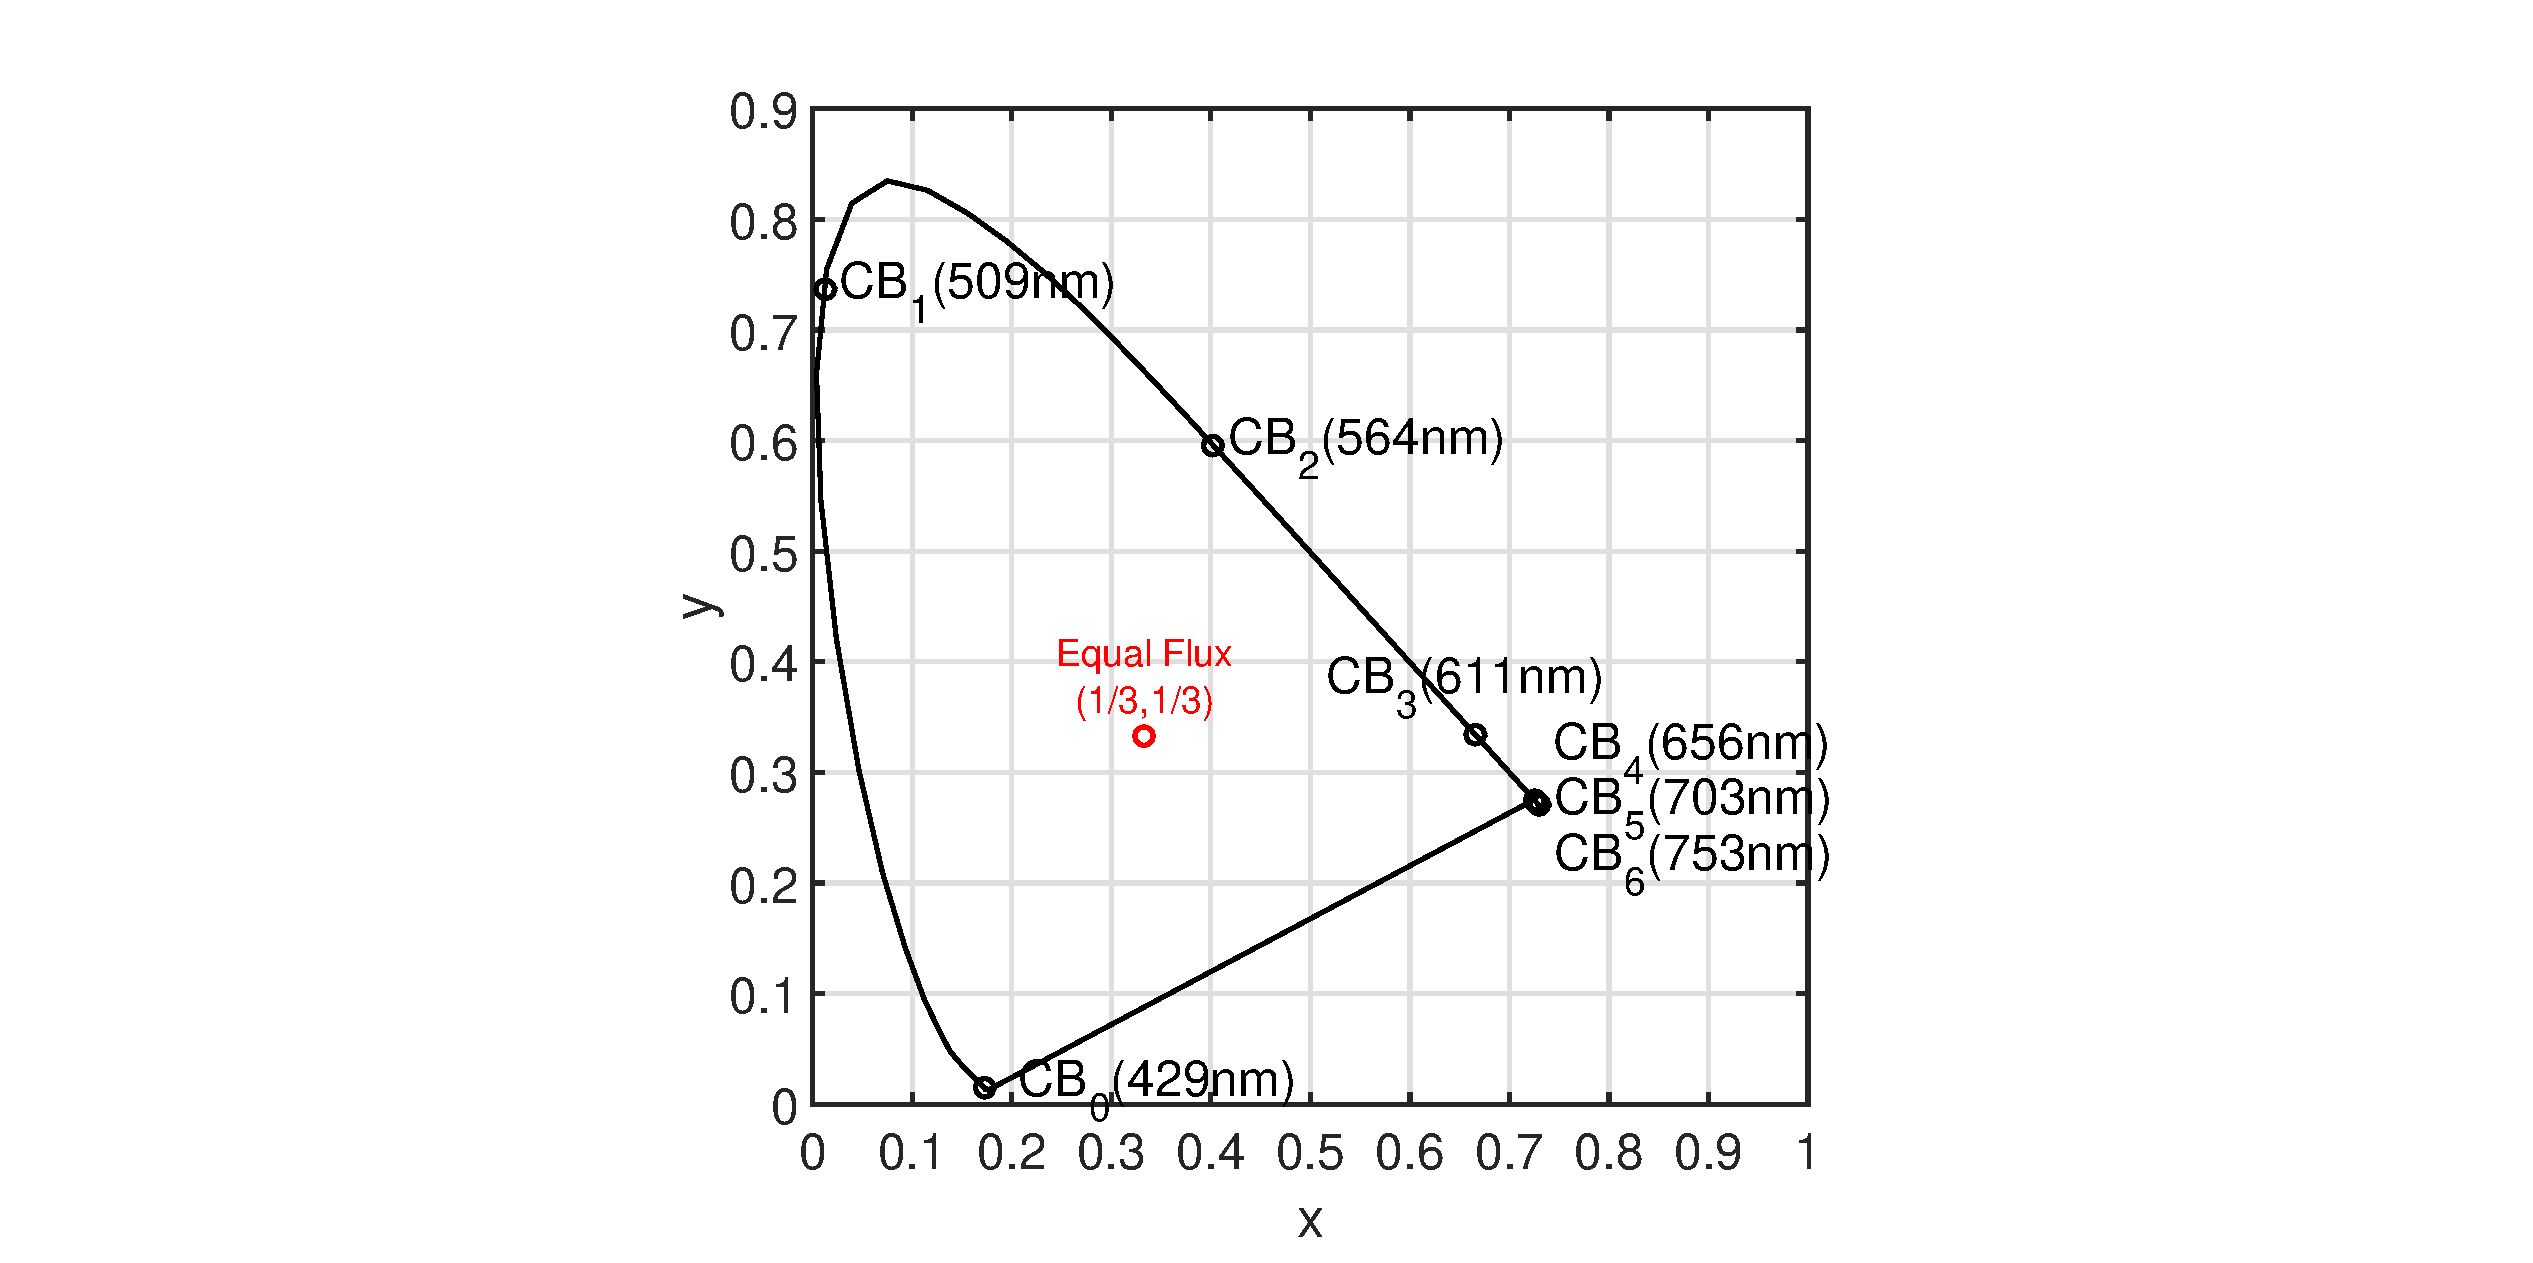
\includegraphics[trim={4.3in 0in 4.3in 0.5in}, clip=true, width=1.9in]{CBCcenters.eps}}
			{\caption{Color band centers on CIE-CS.}}
	\end{floatrow}
\end{figure}
\renewcommand{\arraystretch}{1}

Any SPD within the visible range of
electromagnetic spectrum can produce a stimulus when incident on the
sensors of the human eye (rod and cones) and has a color associated with
it. This color can also be represented by its intensity, hue and
saturation. While intensity is a measure of the total power comprising
the SPD, hue and saturation are subjective parameters analogous to
mean and spread of the wavelengths comprising the SPD and are quantified
by a chromaticity coordinate. The \textit{commission internationale de
  l'eclairage} (CIE) has specified the CIE 1931 XYZ color space (CIE-CS)
that provides a mathematical model to represent the chromaticity of
radiation in the visible range as a point in a 2-dimensional
plane. 
%Monochromatic (saturated) SPDs are represented on the perimeter of the CIE-CS. SPDs emitted by LEDs are usually contain multiple wavelength ranges and are less saturated. As SPDs get increasingly unsaturated, their chromaticity coordinate starts shifting from the perimeter towards coordinate (1/3,1/3). 
Let a luminaire be comprised of three types of LEDs, namely LED$_{n}$; $n\in$ \text{\{i, j, k\}}. The chromaticity of each LED can be
represented by a coordinate ($x_{n}$, $y_{n}$) on the CIE-CS. When
different intensities of radiant flux emitted by three types of LEDs
are combined, the chromaticity coordinate of the resultant SPD will
lie inside the triangle formed by coordinates of the LEDs themselves.
%vertices I ($x_{\text{i}}$,$y_{\text{i}}$), J ($x_{\text{j}}$,$y_{\text{j}}$) and K ($x_{\text{k}}$,$y_{\text{k}}$).

CSK is a modulation technique in which information is transmitted
through changes in chromaticity coordinates. This can be achieved by
varying the intensities of LED$_{n}$ over time. To select sources for CSK implementation, the
standard specifies 7 different color bands -
CB$_{u}$; $0\leq u < 7$ by splicing the visible spectrum range into 7 contiguous
segments as shown in Table 1. The center wavelength of each segment as represented 
on CIE-CS is illustrated in \figurename{ }1. Note that even though center wavelengths of CB$_{4}$, CB$_{5}$ and CB$_{6}$ are 47 nm -- 50 nm apart, the distance between their chromaticity coordinates is very small. The CIE-CS is designed such that the SPD resulting from identical flux emitted by the three primary sources maps to coordinate (1/3, 1/3) which is shown in \figurename{ }1. We can define a color sector on the CIE-CS as the region enclosed by a color band on the perimeter and coordinate (1/3, 1/3). Though not explicitly mentioned in the standard, it is assumed that SPD of
each LED$_{n}$ must belong to a different color sector. To study the performance of CSK independent of specific LED characteristics, it is generally assumed that the
chromaticity coordinate of an LED belonging to a color sector corresponds
to the center wavelength of a color band CB$_{u}$ at the perimeter of the sector as illustrated in \figurename{ }1.

To implement CSK using 3 types of LEDs, the standard defines different
sets of 3 color bands and calls each set a color band combination
(CBC). The 3 different types of LEDs forming a CBC are ordered in a
descending manner based on the center wavelength of the color band
they belong to and each such band is called `band i', `band j' and
`band k' respectively. 9 such CBC$_{v}$; $1\leq v\leq 9$ are defined
in the standard and are outlined in Table \ref{tCBC}. For the rest of
this article, generalized notation CB$^{v}_{n}$ will be used to
indicate color band of type $n\in$ \text{\{i, j, k\}} belonging to CBC$_{v}$. Thus in Table \ref{tCBC}, the cell representing row for CBC$_{v}$ and column for band $n$ provides index $u$ for the color band represented by notation CB$^{v}_{n}$.
Using this notation CB$^{1}_{\text{i}}$ $\equiv$ CB$_{6}$ while CB$^{2}_{\text{j}}$ $\equiv$ CB$_{1}$ and so on.

\begin{table}[b]
\centering
\begin{tabular}{|c|c|c|c|}
\hline
Color band combination & \multicolumn{3}{c|}{Color band '$u$' for CBC$_{v}$} \\
\cline{2-4}
\textbf{CBC$_{v}$} & \textbf{Band i} & \textbf{Band j} & \textbf{Band k} \\
\hline
CBC$_{1}$ & 6 & 2 & 0 \\
\hline
CBC$_{2}$ & 6 & 1 & 0 \\
\hline
CBC$_{3}$ & 5 & 2 & 0 \\
\hline
CBC$_{4}$ & 5 & 1 & 0 \\
\hline
CBC$_{5}$ & 4 & 2 & 0 \\
\hline
CBC$_{6}$ & 4 & 1 & 0 \\
\hline
CBC$_{7}$ & 3 & 2 & 0 \\
\hline
CBC$_{8}$ & 3 & 1 & 0 \\
\hline
CBC$_{9}$ & 2 & 1 & 0 \\
\hline
\end{tabular}
\caption{Color bands combinations as specified by the standard.}
\label{tCBC}
\end{table}

For an $M$-ary CSK using CBC$_{v}$, the design rules to compute the $M$ different constellation points are provided in the standard and their values are outlined in \cite{cskxy}. Let C$^{v}_{n}$ $\equiv$ (x$^{v}_{n}$, y$^{v}_{n}$) be chromaticity coordinate corresponding to CB$^{v}_{n}$. Let C$_{m}$ $\equiv$ ($x_{m}$, $y_{m}$); $0\leq m <$ $M$ be chromaticity coordinate corresponding to m$^{th}$ codeword. Then Table 3 outlines the design rules for computing the constellation points. C$^{v}_{n}$ can be looked up from Table \ref{tCBC} and Table 1. Using these values, remaining C$_{m}$ can then be computed using rules from Table \ref{tMCSK}. Normalized constellation design rules for $M$-ary CSK are illustrated in \figurename{ }\ref{figConst}. Points I, J and K represent normalized coordinates for the $n$ color bands comprising a CBC. 

\begin{table}[t]
\centering
\begin{tabular}{|c|c|c|c|}
\hline
\textbf{m} & \textbf{$M$ = 4} & \textbf{$M$ = 8} & \textbf{$M$ = 16} \\
\hline
0 & C$^{v}_{\text{j}}$ & (2C$_{4}$+C$_{5}$)/3 & C$^{v}_{\text{j}}$\\
1 & (C$^{v}_{\text{i}}$+C$^{v}_{\text{j}}$+C$^{v}_{\text{k}}$)/3 & (2C$_{a}$+C$_{b}$)/3; C$_{a}$=(C$_{b}$+C$_{3}$+C$_{5}$)/3; C$_{b}$=(C$_{4}$+C$_{5}$)/2 & (C$_{0}$+C$_{3}$+C$_{5}$)/3 \\
2 & C$^{v}_{\text{k}}$ & (2C$_{a}$+C$_{b}$)/3; C$_{a}$=(C$_{b}$+C$_{3}$+C$_{7}$)/3; C$_{b}$=(C$_{4}$+C$_{7}$)/2 & (C$_{3}$+C$_{6}$+C$_{10}$)/3 \\
3 & C$^{v}_{\text{i}}$ & (C$_{5}$+C$_{7}$)/2 & (2C$_{0}$+C$_{9}$)/3 \\
\cline{2-2}
4 & & C$^{v}_{\text{j}}$ & (C$_{0}$+2C$_{8}$)/3 \\
5 & & C$^{v}_{\text{k}}$ & (2C$_{0}$+C$_{8}$)/3 \\
6 & & (2C$_{4}$+C$_{7}$)/3 & (C$_{0}$+C$_{8}$+C$_{9}$)/3 \\
7 & & C$^{v}_{\text{i}}$ & (C$_{4}$+C$_{5}$+C$_{6}$)/3 \\
\cline{3-3}
8 & & & C$^{v}_{\text{i}}$ \\
9 & & & C$^{v}_{\text{k}}$ \\
10 & & & (C$_{0}$+2C$_{9}$)/3 \\
11 & & & (C$_{9}$+C$_{10}$+C$_{15}$)/3 \\
12 & & & (2C$_{8}$+C$_{9}$)/3 \\
13 & & & (C$_{4}$+C$_{8}$+C$_{12}$)/3 \\
14 & & & (C$_{6}$+C$_{12}$+C$_{15}$)/3 \\
15 & & & (C$_{8}$+2C$_{9}$)/3 \\
\hline
\end{tabular}
\caption{Design rules to compute constellation points for $M$-ary CSK. Each row computes C$_{m}$, the chromaticity coordinate for m$^{th}$ codeword for any given CBC$_{v}$. C$^{v}_{n}$ is the chromaticity coordinate of color band $n\in$ \{i, j, k\} belonging to CBC$_{v}$.}
\label{tMCSK}
\end{table}

CSK is implemented in conjunction with IM/DD over the optical channel. This channel can be modeled as a linear time invariant system with additive white Gaussian noise (AWGN) and mathematically represented as in Eq.(\ref{eqCHNL})

\begin{equation}
	\vm{Y} = \vm{H}\vm{X} + \vm{W}
	\label{eqCHNL}
\end{equation}
where \vm{X} is an $n_{\text{tx}}$ dimensional vector containing transmit optical powers for each band $n$, \vm{H} is a $n_{\text{rx}}\times n_{\text{tx}}$ dimensional channel matrix, \vm{W} is a $n_{\text{rx}}$ dimensional noise vector and \vm{Y} is an $n_{\text{rx}}$ dimensional receive vector. Channel matrix \vm{H} includes the responsivities of the receive elements.

In $M$-ary CSK, $n_{\text{tx}}=3$ types of LEDs are used to generate $M$ different SPDs corresponding to $M$ different chromaticity coordinates. Each chromaticity coordinate represents a codeword that encodes log$^{ }_{2}$($M$) bits. In order to transmit information, the luminaire irradiates an SPD corresponding to the desired transmit codeword. The clock rate at the luminaire is of the order of tens of MHz. This rate is much higher than which can be perceived by human eye as flicker. In addition, the CSK signaling chain can include a scrambler that ensures data and thus codewords are pseudo-randomly distributed thus mitigating color flicker.

\begin{figure}[b]
	\centering
		\begin{subfigure}{0.32\textwidth}
		\centering
			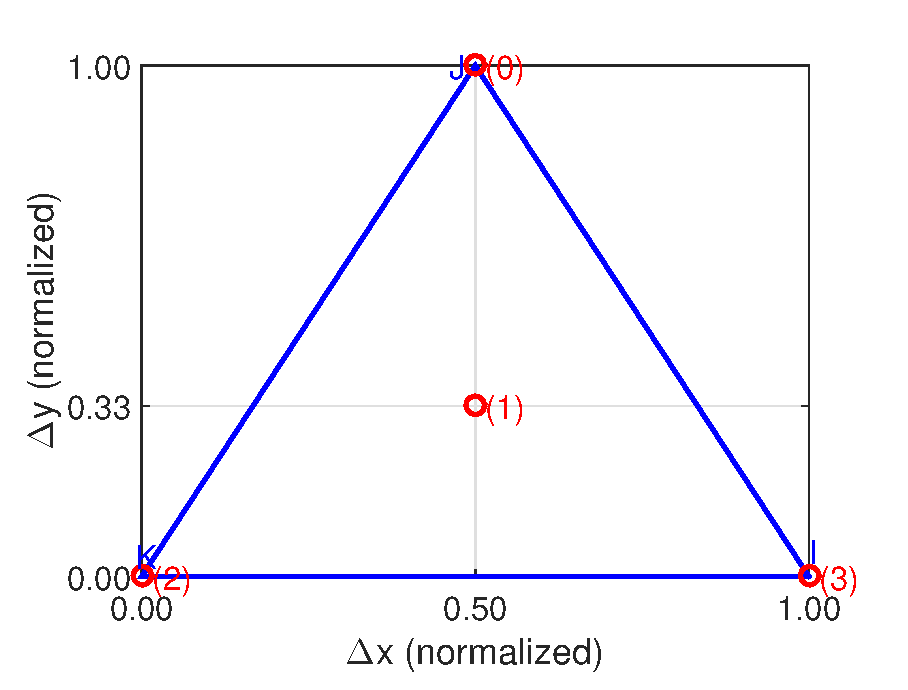
\includegraphics[trim={0.05in 0.0in 0.25in 0.2in}, clip=true, width=\textwidth]{CBCrules4.eps}
			\caption{4-CSK}
			\label{fig4Const}
		\end{subfigure}
		\hfill
		\begin{subfigure}{0.32\textwidth}
		\centering
			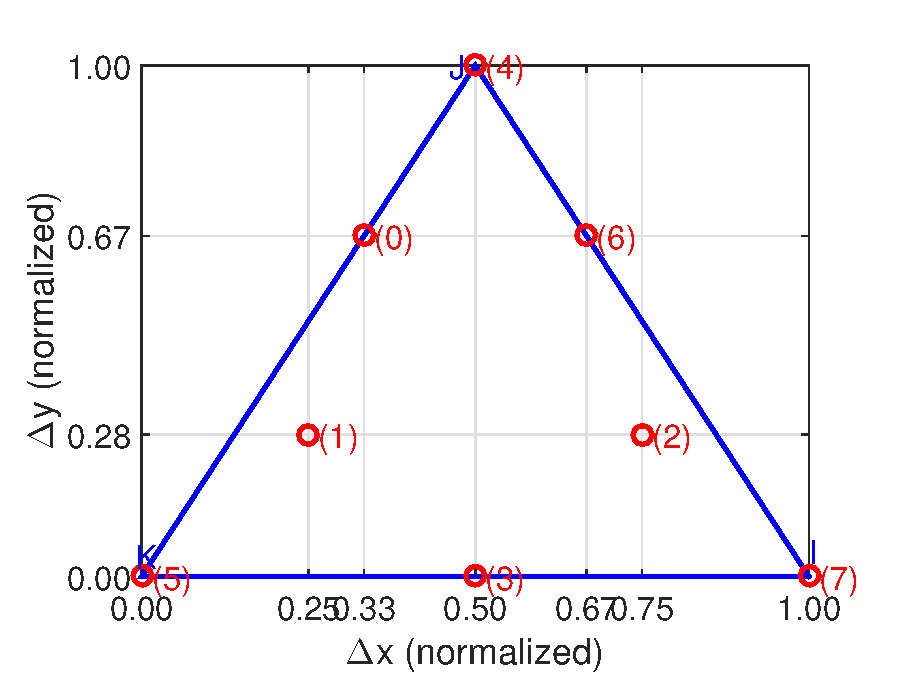
\includegraphics[trim={0.05in 0.0in 0.25in 0.2in}, clip=true, width=\textwidth]{CBCrules8.eps}
			\caption{8-CSK}
			\label{fig8Const}
		\end{subfigure}
		\hfill
		\begin{subfigure}{0.32\textwidth}
		\centering
			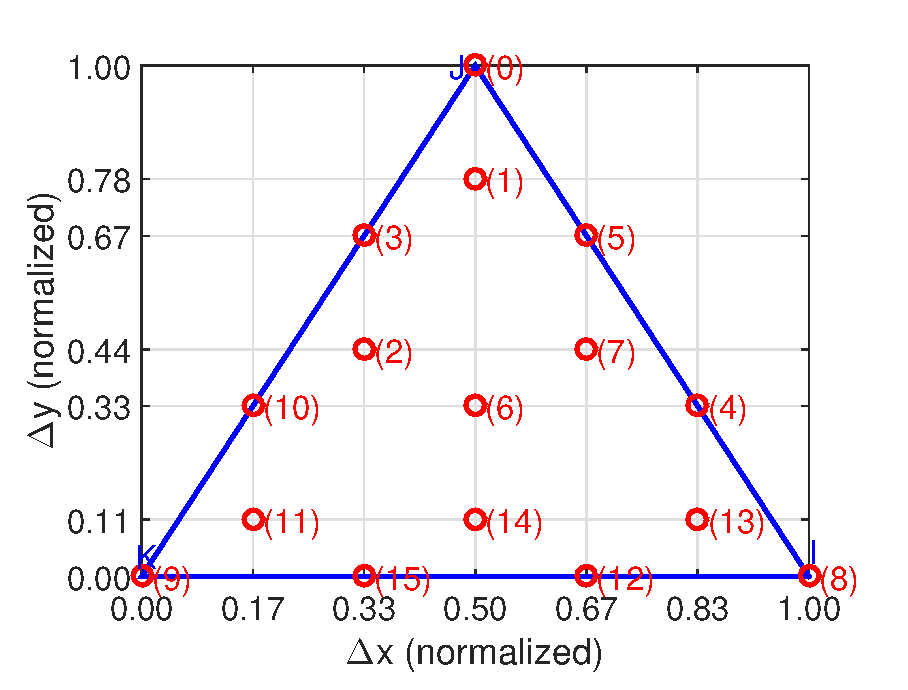
\includegraphics[trim={0.05in 0.0in 0.25in 0.2in}, clip=true, width=\textwidth]{CBCrules16.eps}
			\caption{16-CSK}
			\label{fig16Const}
		\end{subfigure}
	\caption{$M$-ary CSK (normalized) constellation design rules.}
	\label{figConst}
\end{figure}

At the receiving elements, each SPD produces a different electrical response signal. The signal output from each receiving element is corrupted by shot noise of variance $\sigma^{2}_{sh}$ due to ambient light and thermal noise of variance $\sigma^{2}_{th}$ due to trans-impedance amplifier as shown in Eq.(\ref{eqNOISE})

\begin{equation}
	\begin{aligned}
	\sigma^{2}_{sh} &= 2q<i>B\\
	\sigma^{2}_{th} &= \frac{4k_{B}TB}{R_{f}}
\end{aligned}
\label{eqNOISE}
\end{equation}
where $<i>$ is average current generated in the photodiode due incident ambient light, $q$ is charge of an electron, $k_{B}$ is Boltzmann's constant, $T$ is the temperature in Kelvin and $R_{f}$ is the amplifier feedback resistance and B is the channel bandwidth. The signal-to-noise ratio (SNR) can then be defined as in Eq.(\ref{eqSNR})

\begin{equation}
	\text{SNR} \triangleq \frac{\text{Tr}\{\vm{H}\vm{X}\vm{X}^{*}\vm{H}^{*}\}}{\sigma^{2}_{nt}}
	\label{eqSNR}
\end{equation}
where Tr$\{.\}$ is the matrix trace operator, $^{*}$ indicates transpose and $\sigma^{2}_{nt}=\sigma^{2}_{sh}+\sigma^{2}_{th}$ is the total noise variance. SNR in decibel is then computed as 10log$^{ }_{10}$(SNR).

Having received vector \vm{Y}, least squares estimate of transmitted vector ($\hat{\vm{X}}$) can be made by Eq.(\ref{eqXHAT}).
\begin{equation}
	\hat{\vm{X}} = (\vm{H}^{*}\vm{H})^{-1}\vm{H}^{*}\vm{Y}
	\label{eqXHAT}
\end{equation}

After estimating vector $\hat{\vm{X}}$, an estimate of transmitted chromaticity coordinates can be made and transmitted information can then be decoded. The process of transforming chromaticity coordinates to optical power and vice-versa gives rise to two different system models as described in further sections.

%%%%%%%%%%%%%%%%%%%%%  Linear Model  %%%%%%%%%%%%%%%%%%%%%%%
\section{CSK: Linear system model}\label{sCSKL}

The linear CSK model treats the CIE-CS as a linear space to analyze CSK performance. This implies the inherent assumption that when irradiance from multiple transmitting elements is combined, the chromaticity coordinates of the resulting SPD is a linear combination of the chromaticity coordinates of the SPDs of individual transmitting elements. If P$_{n}$; $n\in$ \{i, j, k\} is the normalized radiant flux at the transmit or receive device associated with band $n$, Eq.(\ref{eqLIN}) below taken from the standard provides the implied mathematical relationships between chromaticity coordinates of all bands and that of resultant SPD.

\begin{equation}
	\begin{aligned}
	x_{\text{p}} &= \text{P}_{\text{i}}x_{\text{i}} + \text{P}_{\text{j}}x_{\text{j}} + \text{P}_{\text{k}}x_{\text{k}}\\
	y_{\text{p}} &= \text{P}_{\text{i}}y_{\text{i}} + \text{P}_{\text{j}}y_{\text{j}} + \text{P}_{\text{k}}y_{\text{k}}\\
	1 &= \text{P}_{\text{i}} + \text{P}_{\text{j}} + \text{P}_{\text{k}}
\end{aligned}
\label{eqLIN}
\end{equation}

\begin{figure}[t]
	\centering
		%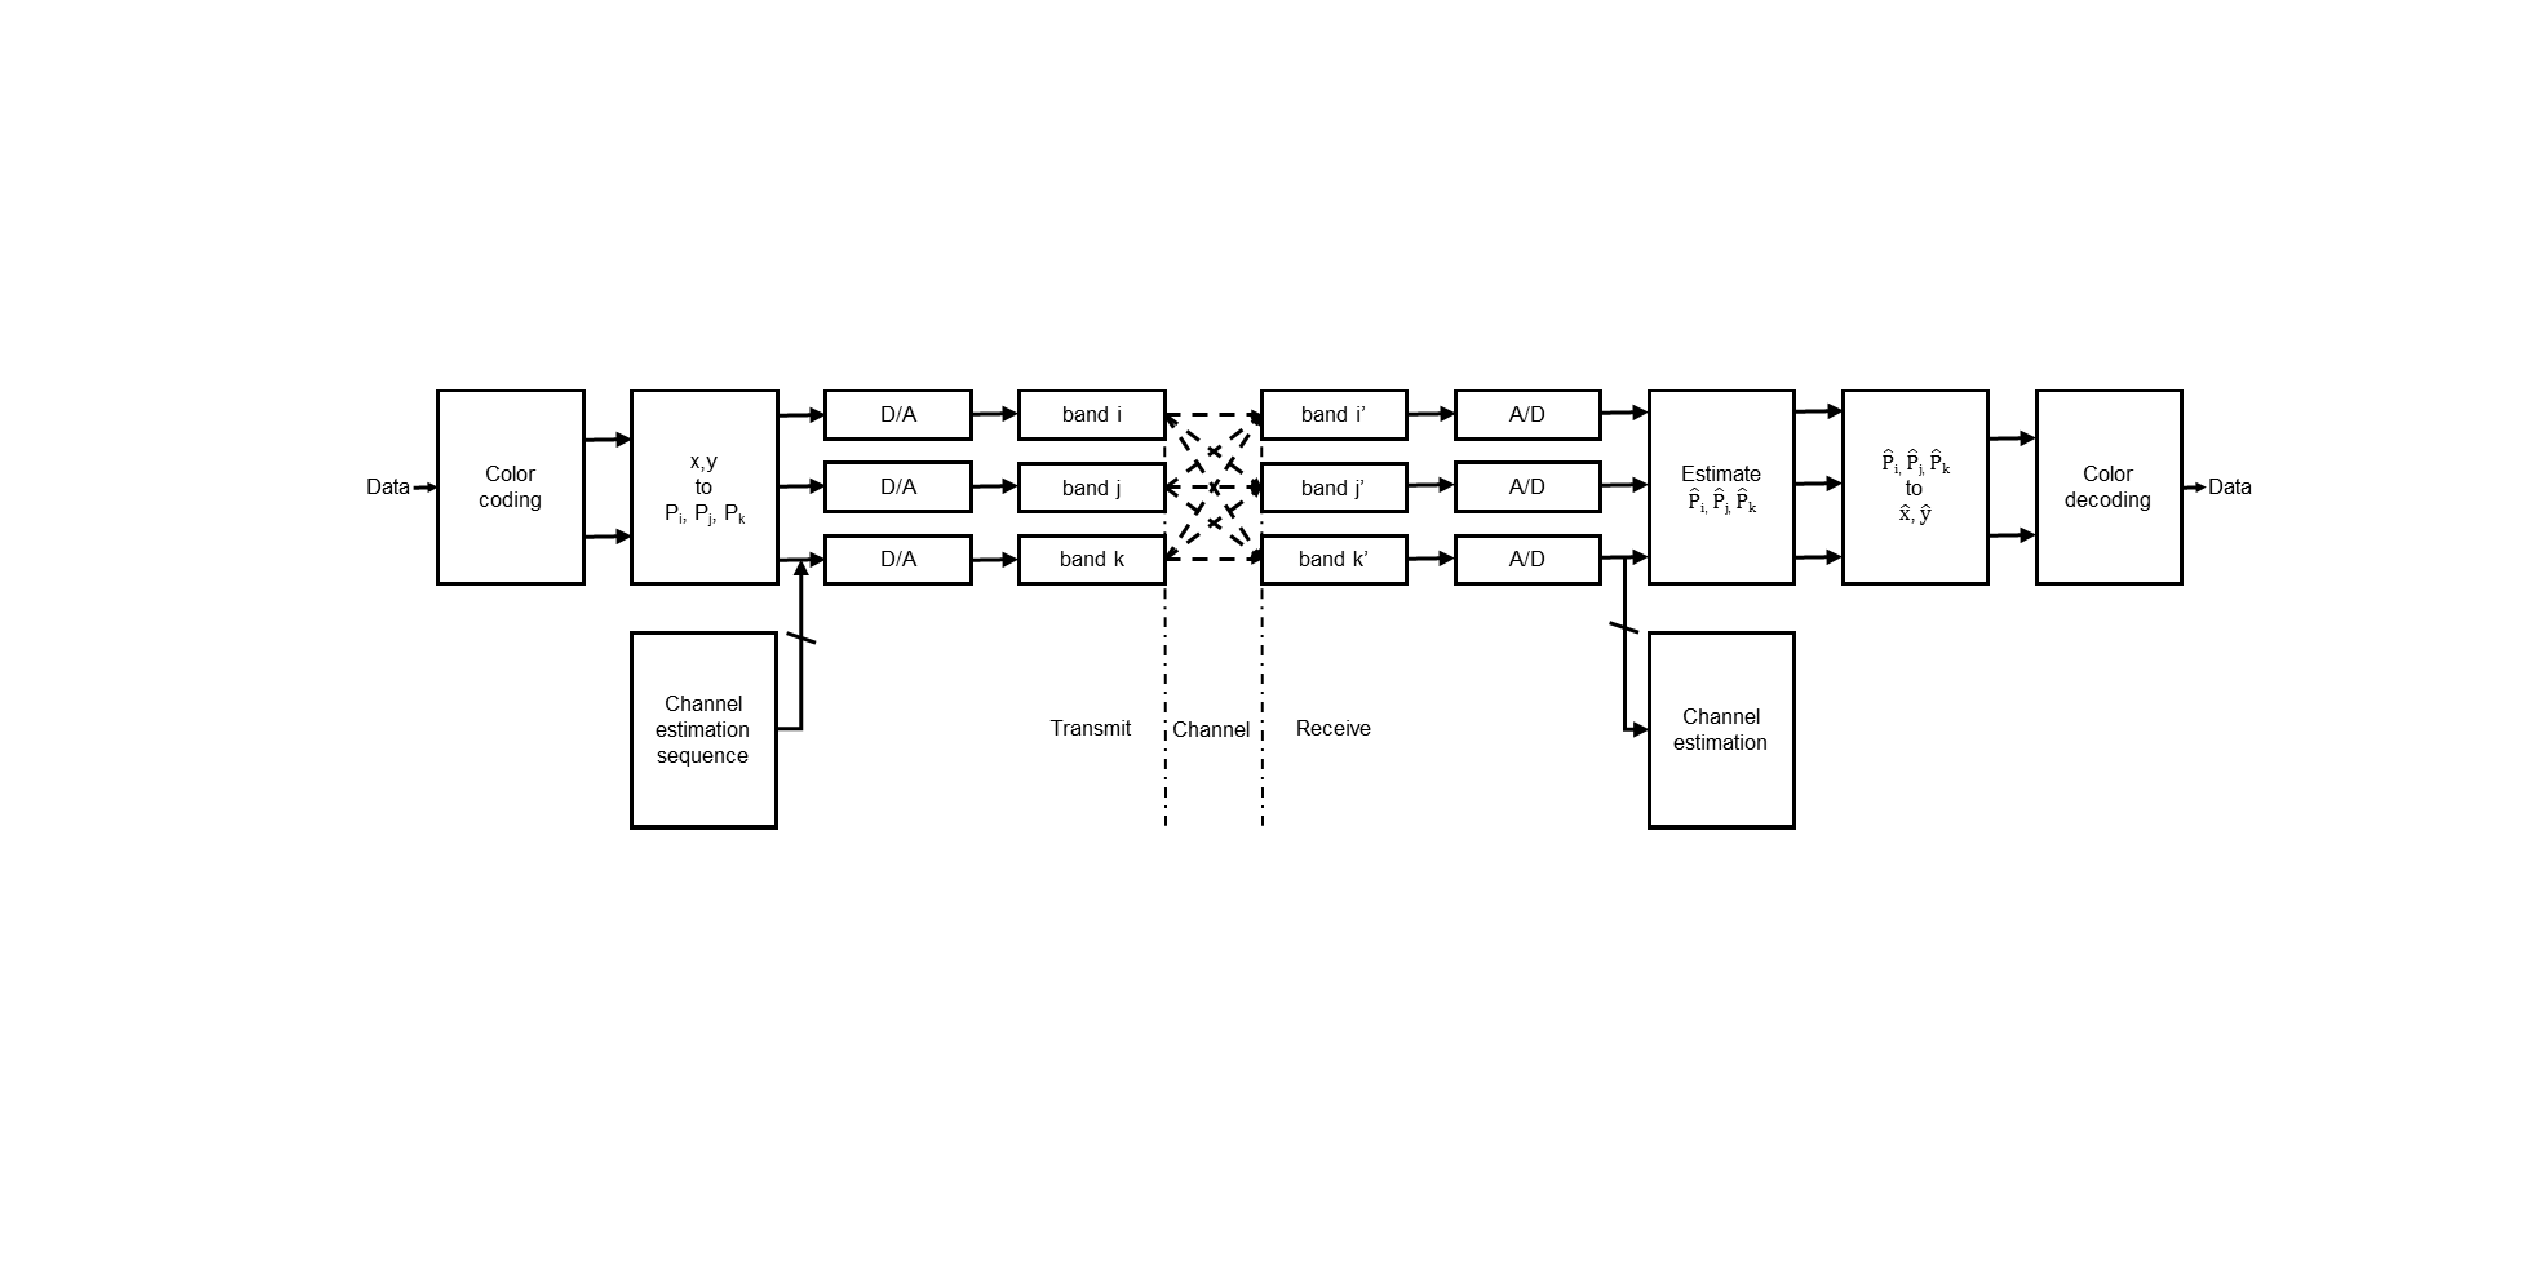
\includegraphics[trim={2.34in 2.78in 1.76in 2.47in}, clip=true, width=5.25in]{CSKBlockDiagram_1.eps}
		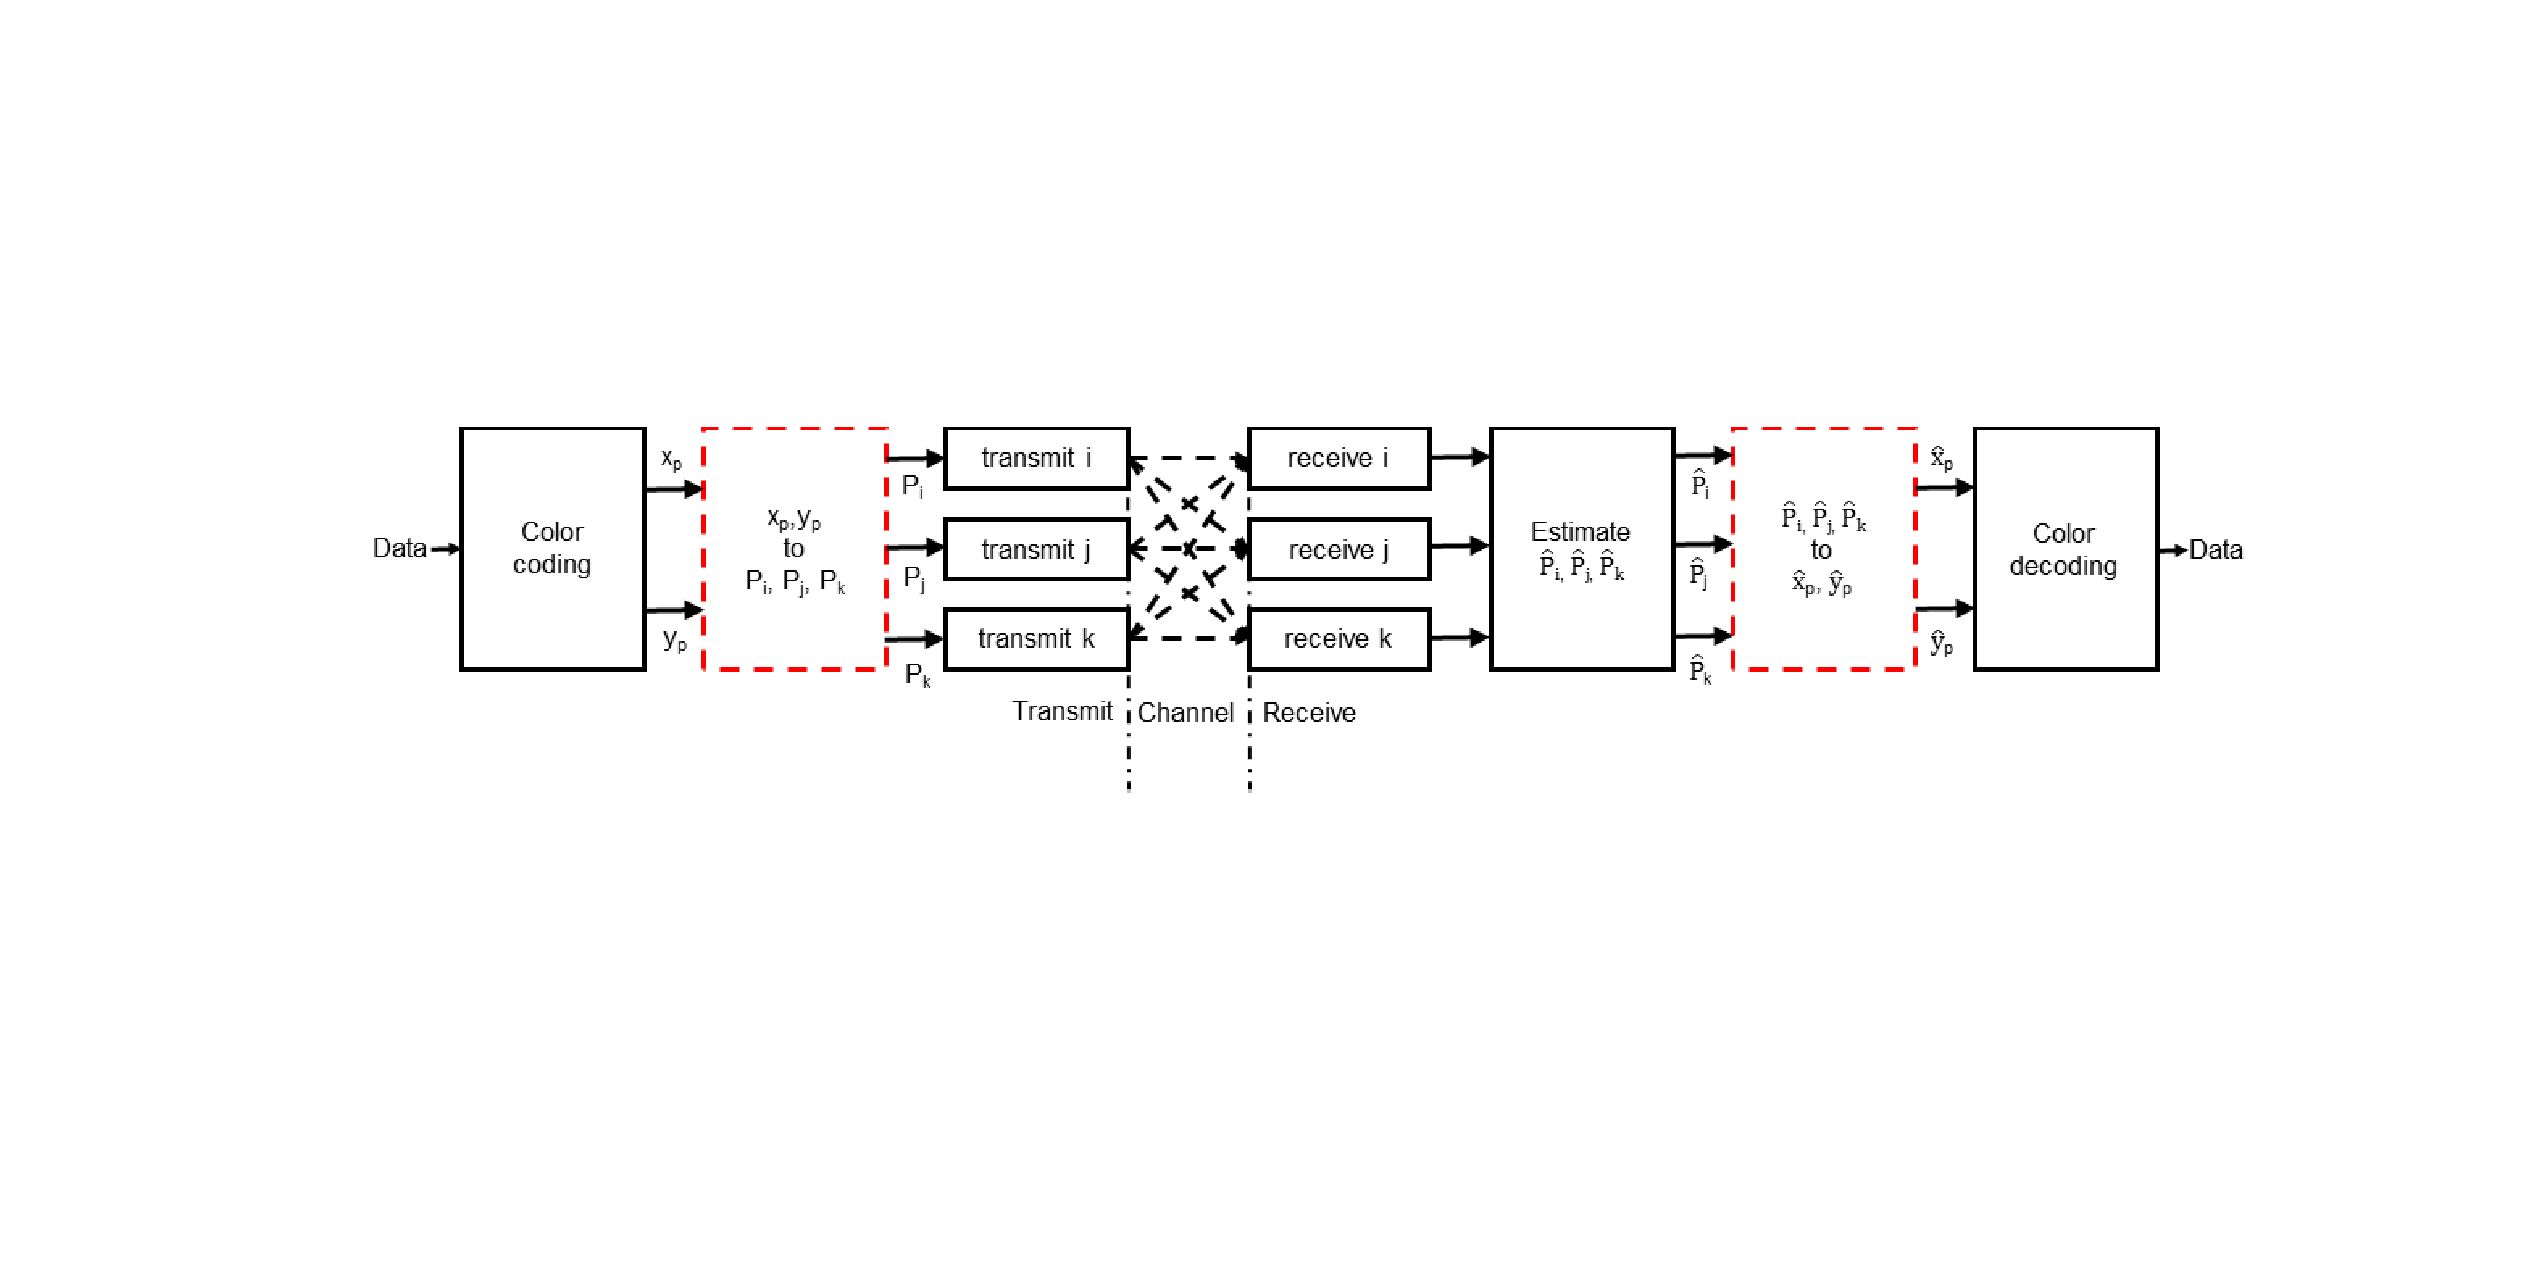
\includegraphics[trim={2.34in 2.78in 1.76in 2.47in}, clip=true, width=5.25in]{CSKBlockDiagram.eps}
	\caption{Block diagram of CSK signal chain. Implementation of red dashed blocks differentiates the linear and the non-linear system models.}
	\label{figCSKBD}
\end{figure}

A block diagram of the CSK signaling chain is shown in \figurename{ }\ref{figCSKBD}. At the transmitting element, the data bit-stream is encoded to chromaticity coordinates ($x_{\text{p}}$, $y_{\text{p}}$) as computed from Table \ref{tMCSK}. Using Eq.(\ref{eqLIN}), normalized P$_{n}$ values are computed which are then scaled to achieve a given illumination target and thus transmit irradiance. A vector of scaled P$_{n}$ values then forms the transmit vector \vm{X}. Without loss of generality, unity electrical to optical conversion at transmitter and unity responsivity (optical to electrical conversion) at the receiver is assumed. Receiving element for band $n$ senses the incident flux and generates an electrical signal proportional to it. AWGN as computed from Eq.\eqref{eqNOISE} is then added to each band $n$ in the form of vector \vm{W}. The receiver output in presence of noise is represented by \vm{Y}. With the knowledge of the channel state and the receiver output, a least squares estimate of transmit vector $\hat{\vm{X}}$ is made using Eq.\eqref{eqXHAT}. Each element of $\hat{\vm{X}}$ then provides the estimates of transmitted flux represented by $\hat{\text{P}}_{n}$. Using these values, ($\hat{x}_{\text{p}}, \hat{y}_{\text{p}}$) are estimated using Eq.\eqref{eqLIN}. Nearest neighbor decoder then estimates the transmitted coordinate and recovers the transmitted information. Thus for the linear system model, Eq.\eqref{eqLIN} represents the ($x_{\text{p}}$, $y_{\text{p}}$) $\rightarrow  \text{P}_{n}$ and $\hat{\text{P}}_{n}\rightarrow$ ($\hat{x}_{\text{p}}$, $\hat{y}_{\text{p}}$) transformations for the red dashed blocks of \figurename{ }\ref{figCSKBD}.
%In this case the channel matrix \vm{H} is $n_{\text{rx}}\times n_{\text{tx}}$ dimensional identity matrix ($n_{\text{rx}}=n_{\text{tx}} = 3$).
  
\begin{figure}[t]
	\centering
		\begin{subfigure}{0.49\textwidth}
		\centering
			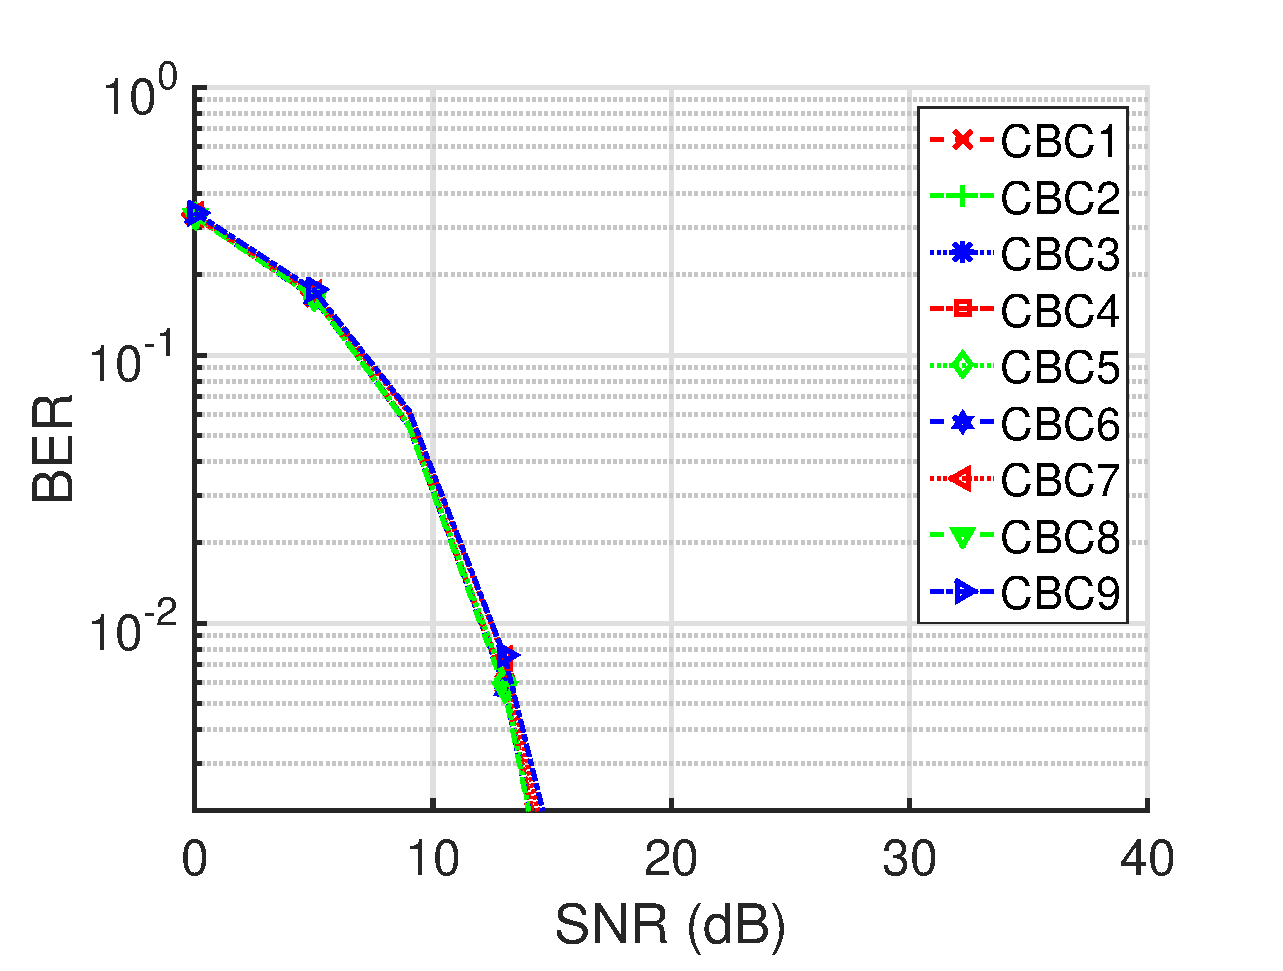
\includegraphics[trim={0.1in 0.0in 0.6in 0.3in}, clip=true, width=\textwidth]{M04_4-CSK_BERvsSNR.eps}
			\caption{4-CSK}
			\label{fig4SNR}
		\end{subfigure}
		\hfill
		\begin{subfigure}{0.49\textwidth}
		\centering
			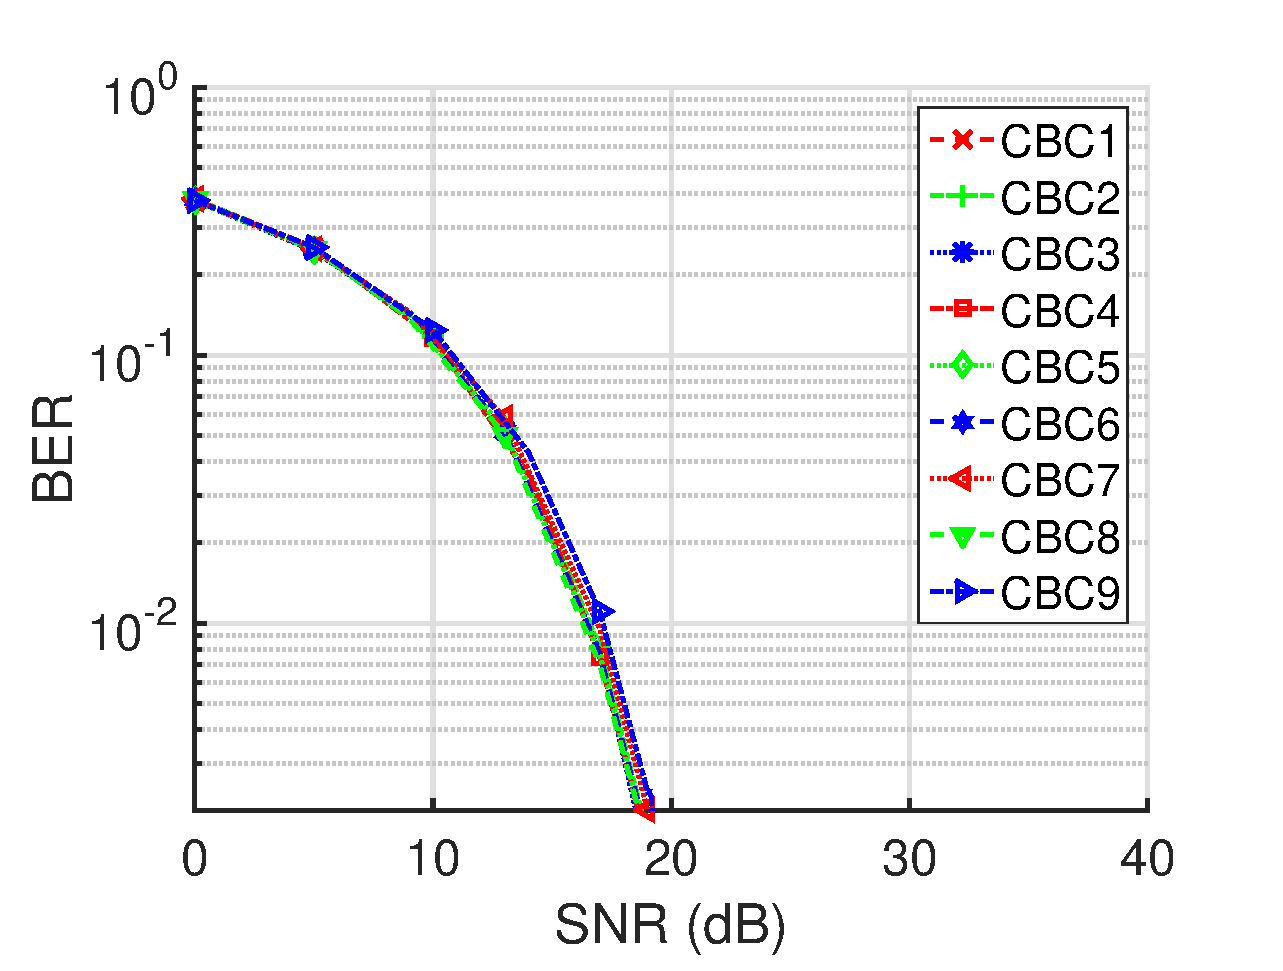
\includegraphics[trim={0.1in 0.0in 0.6in 0.3in}, clip=true, width=\textwidth]{M08_8-CSK_BERvsSNR.eps}
			\caption{8-CSK}
			\label{fig8SNR}
		\end{subfigure}
		\vfill
		\begin{subfigure}{0.49\textwidth}
		\centering
			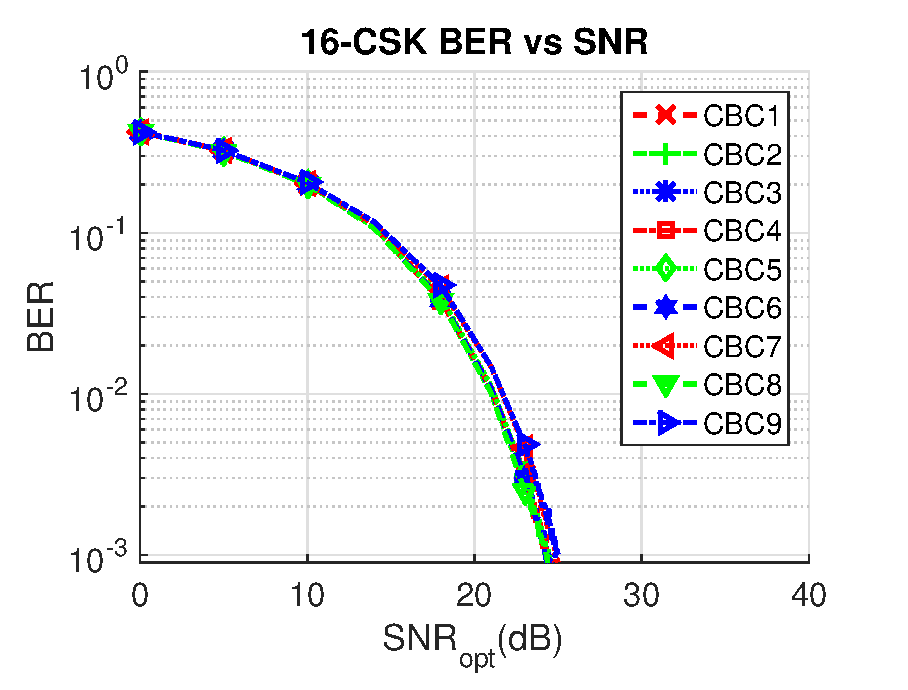
\includegraphics[trim={0.1in 0.0in 0.6in 0.3in}, clip=true, width=\textwidth]{M16_16-CSK_BERvsSNR.eps}
			\caption{16-CSK}
			\label{fig16SNR}
		\end{subfigure}
	\caption{BER vs SNR for linear model}
	\label{figBERvsSNR}
\end{figure}

Monte-carlo simulations are performed to compute performance of $M$-ary CSK under the linear model for all CBC$_{v}$ and \figurename{ }\ref{figBERvsSNR} shows the results. Performance of all CBCs is similar except CBC$_{7}$ and CBC$_{9}$ which perform slightly worse, but only by a margin of about 0.6 dB. This performance is as expected. As seen from Table \ref{tCBC}, CBC$_{7}$ is composed of CB$_{3}$, CB$_{2}$ and CB$_{0}$ whereas and CBC$_{9}$ is composed of CB$_{2}$, CB$_{1}$ and CB$_{0}$. Thus from values in Table 1 and \figurename{ }1, it can be seen that constellation points for other CBCs are the most spread out and have the large minimum distance between constellation points where as that for CBC$_{7}$ and CBC$_{9}$ have the shorter spread and have the smaller minimum distance between constellation points. SNR of at least 15 dB, 20 dB and 25 dB are needed to achieve a target minimum bit error rate (BER) of $10^{-3}$ under the linear model for $M$ = 4, 8 and 16 CSK respectively.

\figurename{ }\ref{figRcvSym} shows received symbols for CBC$_{2}$, whose constellation points are the most spread out, under the linear model. As expected, noise is spread normally along x and y dimensions forming a circular envelop around all constellation points. For $M$ = 8 and $M$ = 16, empty non-interfering regions devoid of received symbols can be seen in the figures. This indicates that these constellations could be better packed by defining additional points in the non-interfering regions. The constellations can then be further optimized to achieve better spectral efficiency. Note that in \figurename{ }\ref{figRcvSym} (\subref{fig4RcvSym}),
(\subref{fig8RcvSym}) and (\subref{fig16RcvSym}), some of the received
symbols are located outside the color gamut (triangle IJK
as outlined in \figurename{ }\ref{figConst}) formed by the sources for
i, j and k bands. This would appear to violate the relationships on the CIE-CS model between coordinates of SPDs of individual sources and that of the resultant SPD formed by mixing the fluxes in different ratios. However, at the receiver, the
received signals are influenced by noise (bipolar, zero-mean Gaussian)
resulting in bipolar received values. Received signals with negative values when mapped back to the CIE-CS, can cause received `noisy' symbols to lie outside of the gamut.

Since the transmitted radiant fluxes are always non-negative, it is possible to clip the receiver output prior to estimating the transmitted
radiant flux.  When negative receiver output is clipped at zero, estimated
symbols are illustrated in
\figurename{ }\ref{figRcvSym} (\subref{fig4RcvSymY0}),
(\subref{fig8RcvSymY0}) and (\subref{fig16RcvSymY0}). This
clipping shows that the mapping back to CIE-CS is sensical. It can also be seen that at target BER of $10^{-3}$, the clipping does not
introduce any significant change in performance when compared to that without clipping.

\begin{figure}[t]
	\centering
		\begin{subfigure}{0.32\textwidth}
		\centering
			\includegraphics[trim={1.0in 0.0in 1.3in 0.1in}, clip=true, width=\textwidth]{M04_4-CSK_CBC2_ReceivedSymbols2.eps}
			\caption{4-CSK}
			\label{fig4RcvSym}
		\end{subfigure}
		\begin{subfigure}{0.32\textwidth}
		\centering
			\includegraphics[trim={1.0in 0.0in 1.3in 0.1in}, clip=true, width=\textwidth]{M08_8-CSK_CBC2_ReceivedSymbols2.eps}
			\caption{8-CSK}
			\label{fig8RcvSym}
		\end{subfigure}
		\begin{subfigure}{0.32\textwidth}
		\centering
			\includegraphics[trim={1.0in 0.0in 1.3in 0.1in}, clip=true, width=\textwidth]{M16_16-CSK_CBC2_ReceivedSymbols3.eps}
			\caption{16-CSK}
			\label{fig16RcvSym}
		\end{subfigure}
		%%%%%%%%% Y0 %%%%%%%%%
		\begin{subfigure}{0.32\textwidth}
		\centering
			\includegraphics[trim={1.0in 0.0in 1.3in 0.1in}, clip=true, width=\textwidth]{M04_4-CSK_CBC2_ReceivedSymbols2_Y0.eps}
			\caption{4-CSK}
			\label{fig4RcvSymY0}
		\end{subfigure}
		\begin{subfigure}{0.32\textwidth}
		\centering
			\includegraphics[trim={1.0in 0.0in 1.3in 0.1in}, clip=true, width=\textwidth]{M08_8-CSK_CBC2_ReceivedSymbols2_Y0.eps}
			\caption{8-CSK}
			\label{fig8RcvSymY0}
		\end{subfigure}
		\begin{subfigure}{0.32\textwidth}
		\centering
			\includegraphics[trim={1.0in 0.0in 1.3in 0.1in}, clip=true, width=\textwidth]{M16_16-CSK_CBC2_ReceivedSymbols3_Y0.eps}
			\caption{16-CSK}
			\label{fig16RcvSymY0}
		\end{subfigure}
	\caption{Received symbols for CBC$_{2}$. (\subref{fig4RcvSym}),(\subref{fig8RcvSym}),(\subref{fig16RcvSym}): Receiver output not clipped. (\subref{fig4RcvSymY0}),(\subref{fig8RcvSymY0}),(\subref{fig16RcvSymY0}): Negative values of receiver output clipped at zero.}
	\label{figRcvSym}
\end{figure}

While this linear system model is instructive to study $M$-ary CSK modulation
and carry out a first order performance analysis, a practical CSK
system incorporating human eye's visual perception, is non-linear due to non-linearity of the CIE-CS. The ($x_{\text{p}}$, $y_{\text{p}}$) $\rightarrow  \text{P}_{n}$ block at the transmitter and its counterpart and $\hat{\text{P}}_{n}\rightarrow$ ($\hat{x}_{\text{p}}$, $\hat{y}_{\text{p}}$) at the receiver (red colored dashed
blocks in \figurename{ }\ref{figCSKBD}) introduce this non-linearity
which significantly alters the $M$-ary CSK performance for a practical
implementation. The effects of these practical constraints on a CSK
system are studied in next few sections.

%%%%%%%%%%%%%%%%%%%  Non-linear Model  %%%%%%%%%%%%%%%%%%%%%
\section{CSK: Non-linear system model}\label{sCSKNL}

To understand the source of non-linearity in the CSK system, let's take a look at the CIE-CS which empirically models the human eye's visual perception of color for a stimulating SPD. Let $S_{n}(\lambda)$ be the SPDs of the transmit LEDs and P$_{n}$ be the radiant flux associated with band $n$. Thus the aggregate transmitted SPD is given by Eq.\eqref{eqWLDA}.

\begin{figure}[b]
	\centering
		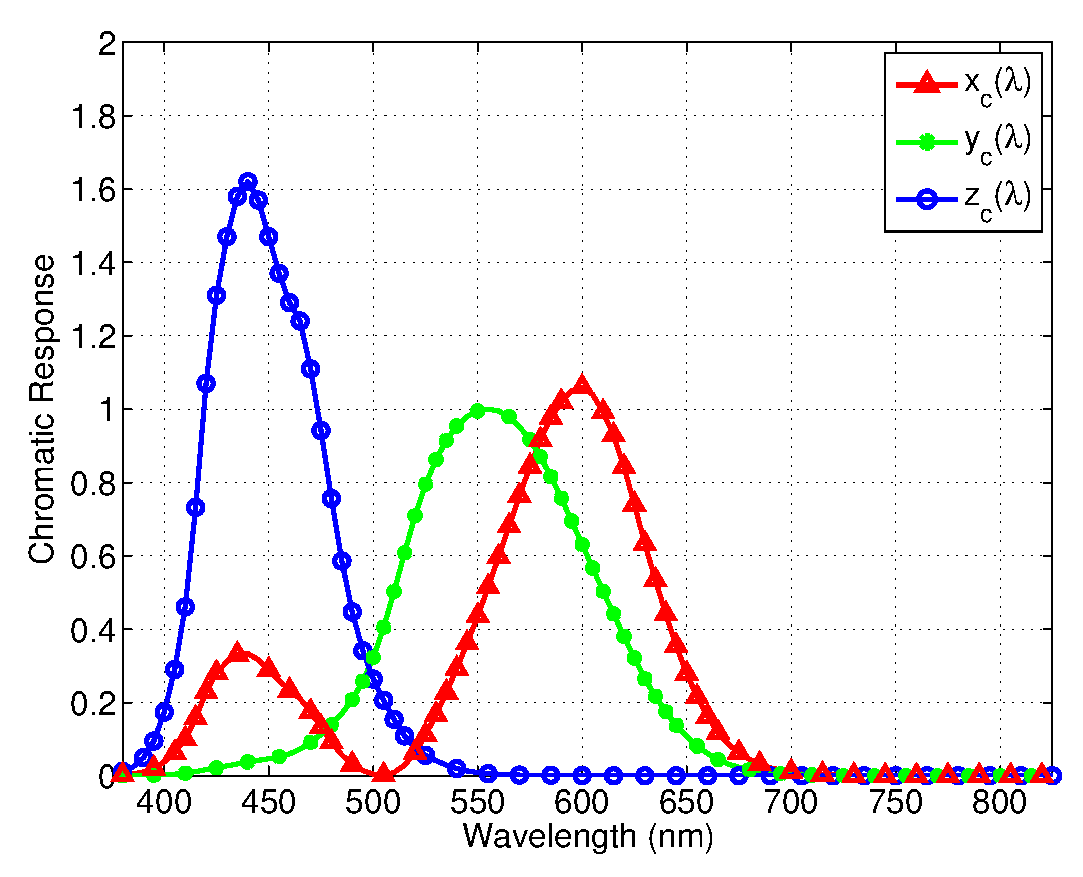
\includegraphics[trim={0.05in 0.05in 0.05in 0.05in}, clip=true, width=2.4in]{CIE1931CMF.eps}
	\caption{CIE 1931 XYZ color matching functions.}
	\label{figCIEXYZ}
\end{figure}

\begin{equation}
	W(\lambda) = \sum\limits_{n\text{ }\in\text{ \{i, j, k\}}}\text{P}_{n}S_{n}(\lambda)
	\label{eqWLDA}
\end{equation}

CIE-CS specification outlines three color matching functions - $x_{c}(\lambda)$, $y_{c}(\lambda)$ and $z_{c}(\lambda)$ as illustrated in \figurename{ }\ref{figCIEXYZ}. The tristimulus values for the three primary sources as defined in the CIE-CS are given by Eq.\eqref{eqTXYZ} and the chromaticity coordinates ($x_{\text{p}}$, $y_{\text{p}}$) of the resultant SPD $W(\lambda)$ are given by Eq.\eqref{eqWXY}. From Eqs.(\ref{eqWLDA}-\ref{eqWXY}) it can also be inferred that the relationship between P$_{n}$ and ($x_{\text{p}}$, $y_{\text{p}}$) is non-linear.

\begin{equation}
	\begin{aligned}
		X_{W} &= \int\limits_{\lambda\text{ = 380 nm}}^{\lambda\text{ = 780 nm}}W(\lambda)x_{c}(\lambda)d\lambda\\
		Y_{W} &= \int\limits_{\lambda\text{ = 380 nm}}^{\lambda\text{ = 780 nm}}W(\lambda)y_{c}(\lambda)d\lambda\\
		Z_{W} &= \int\limits_{\lambda\text{ = 380 nm}}^{\lambda\text{ = 780 nm}}W(\lambda)z_{c}(\lambda)d\lambda
	\end{aligned}
	\label{eqTXYZ}
\end{equation}

\begin{equation}
	x_{\text{p}} = \frac{X_{W}}{X_{W}+Y_{W}+Z_{W}}; \text{  } y_{\text{p}} = \frac{Y_{W}}{X_{W}+Y_{W}+Z_{W}} % \text{  } adds space.
	\label{eqWXY}
\end{equation}

\begin{figure}[t]
	\centering
		\begin{subfigure}{0.49\textwidth}
		\centering
			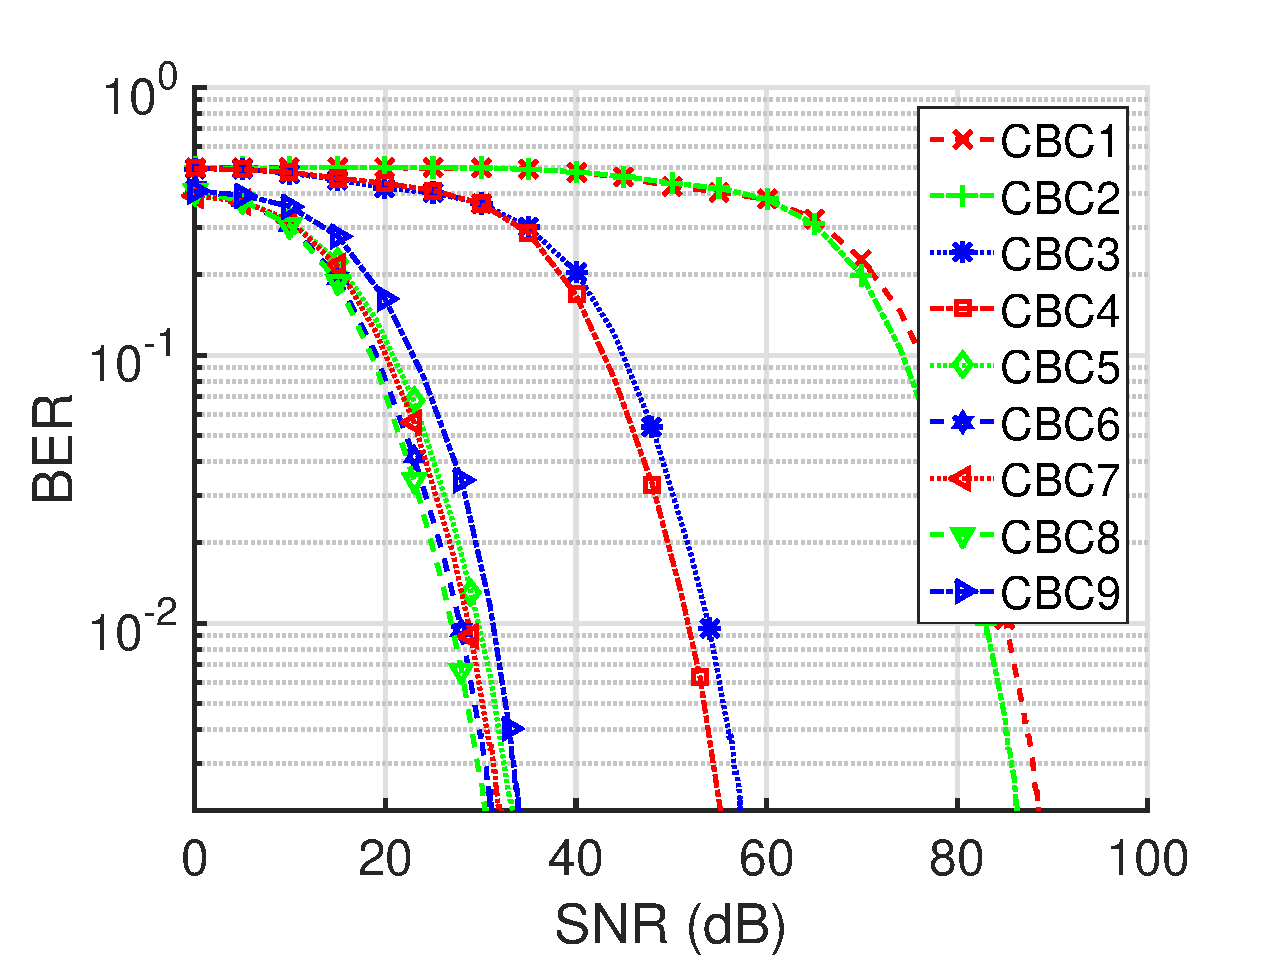
\includegraphics[trim={0.1in 0.0in 0.5in 0.3in}, clip=true, width=\textwidth]{M04_4-CSK_BERvsSNR_NL.eps}
			\caption{4-CSK}
			\label{fig4SNR_NL}
		\end{subfigure}
		\hfill
		\begin{subfigure}{0.49\textwidth}
		\centering
			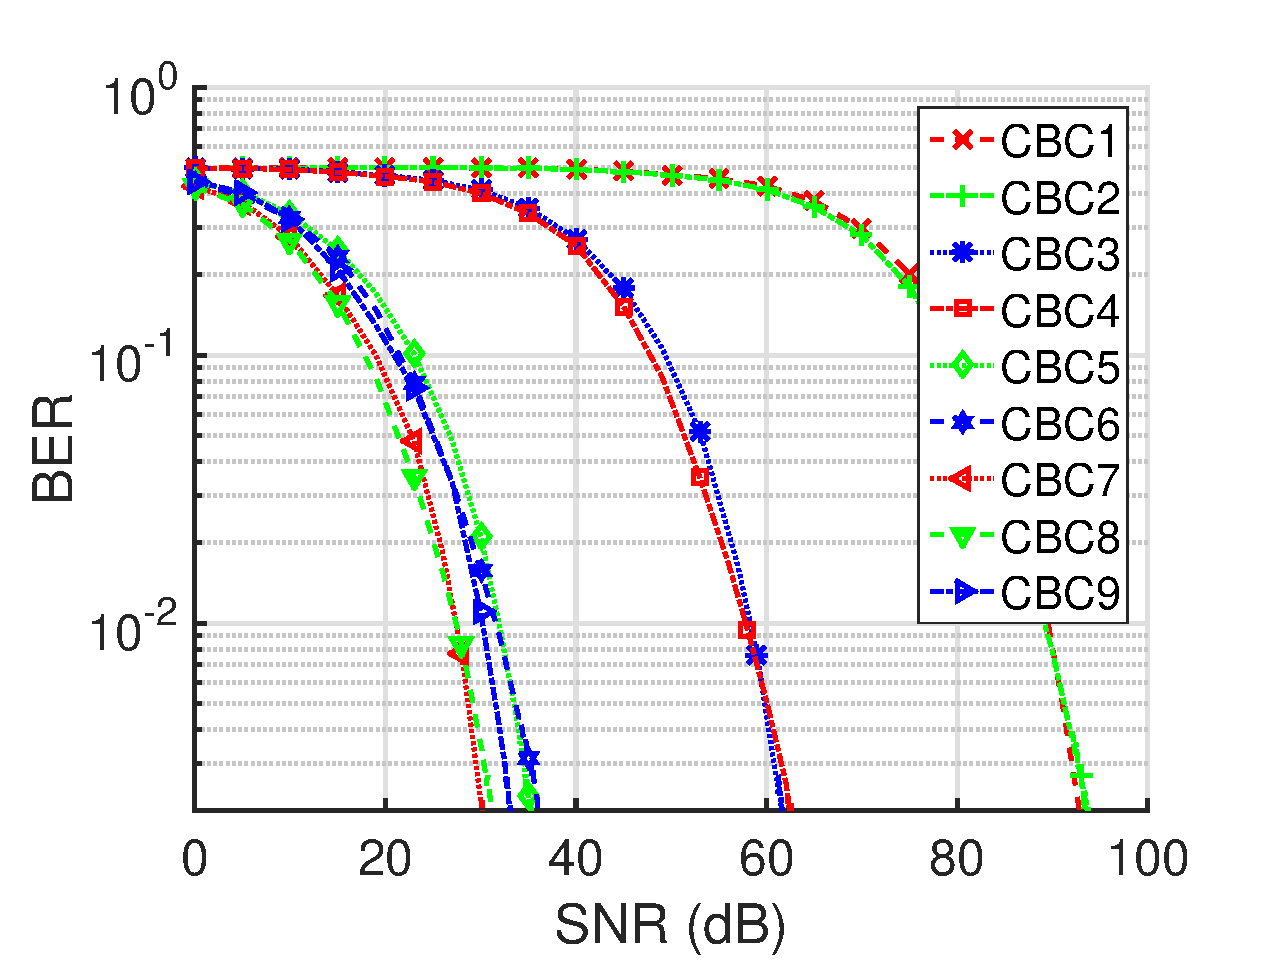
\includegraphics[trim={0.1in 0.0in 0.5in 0.3in}, clip=true, width=\textwidth]{M08_8-CSK_BERvsSNR_NL.eps}
			\caption{8-CSK}
			\label{fig8SNR_NL}
		\end{subfigure}
		\vfill
		\begin{subfigure}{0.49\textwidth}
		\centering
			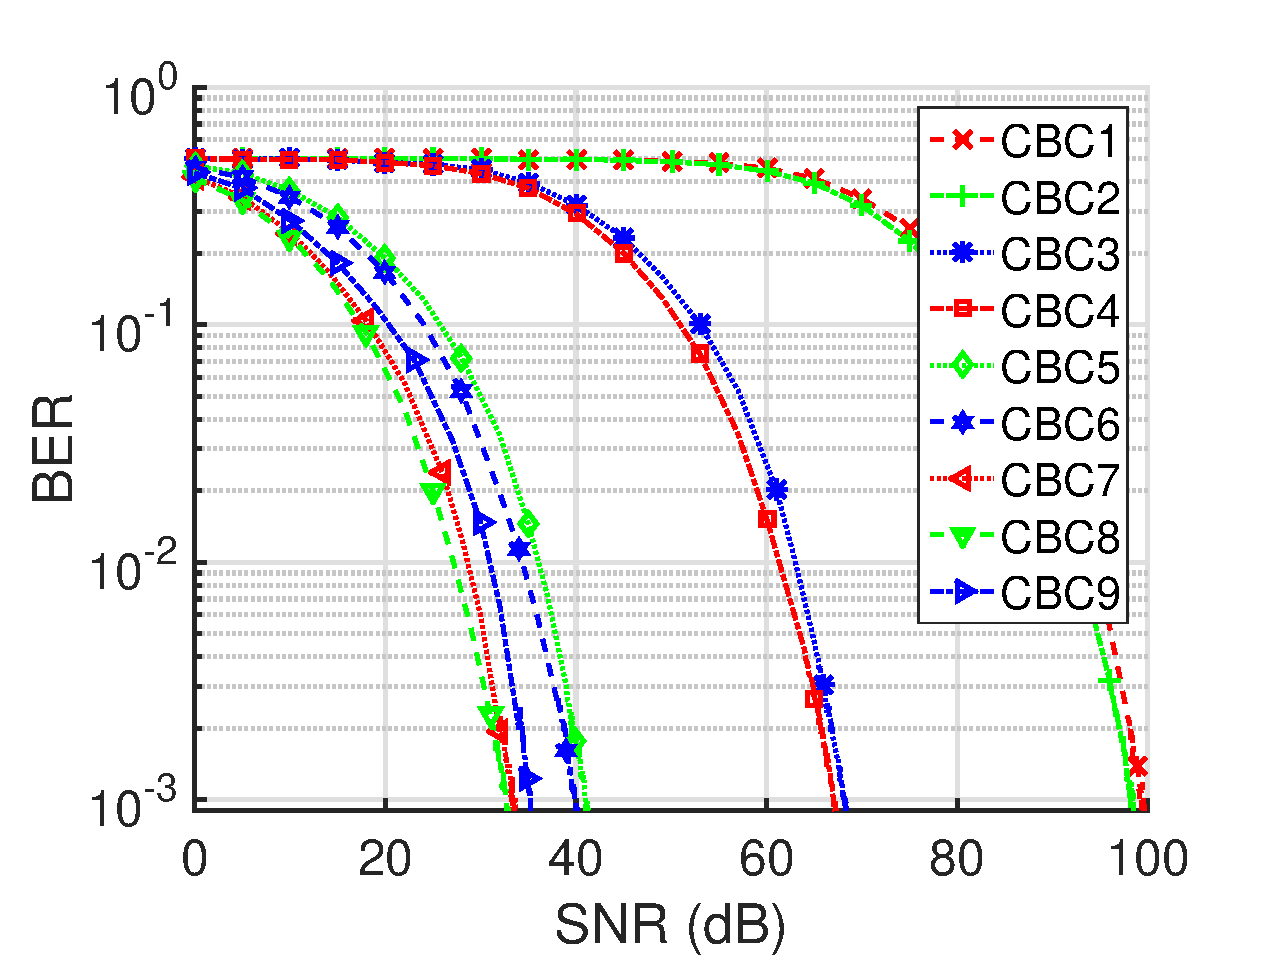
\includegraphics[trim={0.1in 0.0in 0.5in 0.3in}, clip=true, width=\textwidth]{M16_16-CSK_BERvsSNR_NL.eps}
			\caption{16-CSK}
			\label{fig16SNR_NL}
		\end{subfigure}
	\caption{BER vs SNR for all CBC}
	\label{figBERvsSNR_NL}
\end{figure}

As outlined in prior sections, $M$-ary CSK modulation transmits information by varying the chromaticity coordinates of transmit SPD. In a practical implementation, a table of unique transformation ratios P$_{\text{i}}$:P$_{\text{j}}$:P$_{\text{k}}$ $\rightarrow$ $(x_{\text{p}},y_{\text{p}})$ can be pre-computed for each of the $M$ constellation points. Referring back to \figurename{ }\ref{figCSKBD}, at the transmitter the data is color coded to obtain ($x_{\text{p}}$, $y_{\text{p}}$) coordinate to transmit. Given this coordinate, corresponding flux ratios P$_{\text{i}}$:P$_{\text{j}}$:P$_{\text{k}}$ can be looked up from the pre-computed table. The target illumination requirements provide the total radiant flux to output from the transmitting sources. With the flux ratio and the total radiant flux information, individual P$_{n}$ for each band $n$ can now be computed from Eq.\eqref{eqWLDA}. This transformation now forms the ($x_{\text{p}}$, $y_{\text{p}}$) $\rightarrow  \text{P}_{n}$ block in the transmitter signaling chain. These transmitted flux are sensed by the receivers in presence of AWGN. The receivers generate an electrical output which is then used to compute an estimate of transmitted radiant fluxes $\hat{\text{P}}_{n}$. Eqs.(\ref{eqWLDA}-\ref{eqWXY}), which now constitute the $\hat{\text{P}}_{n}\rightarrow$ ($\hat{x}_{\text{p}}$, $\hat{y}_{\text{p}}$) block in the receive signal chain, can then be used to estimate the transmitted coordinate ($\hat{x}_{\text{p}}$, $\hat{y}_{\text{p}}$). Thus, the AWGN added to the received signal undergoes a non-linear transformation during $\hat{\text{P}}_{n}\rightarrow$ ($\hat{x}_{\text{p}}$, $\hat{y}_{\text{p}}$) process which skews the noise in the chromaticity plane of the CIE-CS. This causes additional performance penalties in a practical CSK system.

%MAKE indivual letters below into math? Italic?

\figurename{ }\ref{figBERvsSNR_NL} shows performance of all the CBCs under this non-linear model. These curves are obtained by monte-carlo simulations similar to those performed for the linear model after substituting the P$_{n}$ $\rightarrow$ ($x_{\text{p}}$, $y_{\text{p}}$) and $\hat{\text{P}}_{n}\rightarrow$ ($\hat{x}_{\text{p}}$, $\hat{y}_{\text{p}}$) blocks with the non-linear system model transformations. It can be observed that CBC$_{7}$ and CBC$_{8}$ perform relatively similar and are the best while CBC$_{1}$ performs the worst. Additionally, it is observed that CBC$_{1}$-CBC$_{4}$ perform significantly worse as compared to the rest. For CBC$_{1}$-CBC$_{4}$, the amount of radiant flux emitted by band i is 3-4 orders of magnitude greater than band j and 1-2 orders of magnitude greater than band k. Thus the $\hat{\text{P}}_{n}\rightarrow$ ($\hat{x}_{\text{p}}$, $\hat{y}_{\text{p}}$) conversion at the receiver is extremely sensitive to noise along the j and k bands as compared to that along the i band. This introduces significant errors in decoding received symbols.

\begin{figure}[t]
	\centering
		%%%%%%%%% CBC1 %%%%%
		\begin{subfigure}{0.32\textwidth}
		\centering
			\includegraphics[trim={1.0in 0.0in 1.3in 0.1in}, clip=true, width=\textwidth]{M04_4-CSK_CBC1_ReceivedSymbols9_NL.eps}
			\caption{CBC$_{1}$: 4-CSK}
			\label{fig4RcvSym_NL1}
		\end{subfigure}
		\hfill
		\begin{subfigure}{0.32\textwidth}
		\centering
			\includegraphics[trim={1.0in 0.0in 1.3in 0.1in}, clip=true, width=\textwidth]{M08_8-CSK_CBC1_ReceivedSymbols10_NL.eps}
			\caption{CBC$_{1}$: 8-CSK}
			\label{fig8RcvSym_NL1}
		\end{subfigure}
		\hfill
		\begin{subfigure}{0.32\textwidth}
		\centering
			\includegraphics[trim={1.0in 0.0in 1.3in 0.1in}, clip=true, width=\textwidth]{M16_16-CSK_CBC1_ReceivedSymbols10_NL.eps}
			\caption{CBC$_{1}$: 16-CSK}
			\label{fig16RcvSym_NL1}
		\end{subfigure}
		\vfill
		%%%%%%%%% CBC8 %%%%%
		\begin{subfigure}{0.32\textwidth}
		\centering
			\includegraphics[trim={1.0in 0.0in 1.3in 0.1in}, clip=true, width=\textwidth]{M04_4-CSK_CBC8_ReceivedSymbols4_NL.eps}
			\caption{CBC$_{8}$: 4-CSK}
			\label{fig4RcvSym_NL8}
		\end{subfigure}
		\hfill
		\begin{subfigure}{0.32\textwidth}
		\centering
			\includegraphics[trim={1.0in 0.0in 1.3in 0.1in}, clip=true, width=\textwidth]{M08_8-CSK_CBC8_ReceivedSymbols4_NL.eps}
			\caption{CBC$_{8}$: 8-CSK}
			\label{fig8RcvSym_NL8}
		\end{subfigure}
		\hfill
		\begin{subfigure}{0.32\textwidth}
		\centering
			\includegraphics[trim={1.0in 0.0in 1.3in 0.1in}, clip=true, width=\textwidth]{M16_16-CSK_CBC8_ReceivedSymbols4_NL.eps}
			\caption{CBC$_{8}$: 16-CSK}
			\label{fig16RcvSym_NL8}
		\end{subfigure}
	\caption{Received symbols for non-linear model when receiver output is not clipped. Some received symbols are located outside the color gamut. Note that noise when transformed to chromaticity plane is no longer AWGN.}
	\label{figRcvSym_NL}
\end{figure}

\begin{figure}[t]
	\centering
	%%%%%%%%% CBC1 Y0 %%%%%
		\begin{subfigure}{0.32\textwidth}
		\centering
			\includegraphics[trim={1.0in 0.0in 1.3in 0.1in}, clip=true, width=\textwidth]{M04_4-CSK_CBC1_ReceivedSymbols9_NL_Y0.eps}
			\caption{CBC$_{1}$: 4-CSK}
			\label{fig4RcvSym_NL1_Y0}
		\end{subfigure}
		\hfill
		\begin{subfigure}{0.32\textwidth}
		\centering
			\includegraphics[trim={1.0in 0.0in 1.3in 0.1in}, clip=true, width=\textwidth]{M08_8-CSK_CBC1_ReceivedSymbols10_NL_Y0.eps}
			\caption{CBC$_{1}$: 8-CSK}
			\label{fig8RcvSym_NL1_Y0}
		\end{subfigure}
		\hfill
		\begin{subfigure}{0.32\textwidth}
		\centering
			\includegraphics[trim={1.0in 0.0in 1.3in 0.1in}, clip=true, width=\textwidth]{M16_16-CSK_CBC1_ReceivedSymbols10_NL_Y0.eps}
			\caption{CBC$_{1}$: 16-CSK}
			\label{fig16RcvSym_NL1_Y0}
		\end{subfigure}
		\vfill
		%%%%%%%%% CBC8 Y0 %%%%%
		\begin{subfigure}{0.32\textwidth}
		\centering
			\includegraphics[trim={1.0in 0.0in 1.3in 0.1in}, clip=true, width=\textwidth]{M04_4-CSK_CBC8_ReceivedSymbols4_NL_Y0.eps}
			\caption{CBC$_{8}$: 4-CSK}
			\label{fig4RcvSym_NL8_Y0}
		\end{subfigure}
		\hfill
		\begin{subfigure}{0.32\textwidth}
		\centering
			\includegraphics[trim={1.0in 0.0in 1.3in 0.1in}, clip=true, width=\textwidth]{M08_8-CSK_CBC8_ReceivedSymbols4_NL_Y0.eps}
			\caption{CBC$_{8}$: 8-CSK}
			\label{fig8RcvSym_NL8_Y0}
		\end{subfigure}
		\hfill
		\begin{subfigure}{0.32\textwidth}
		\centering
			\includegraphics[trim={1.0in 0.0in 1.3in 0.1in}, clip=true, width=\textwidth]{M16_16-CSK_CBC8_ReceivedSymbols4_NL_Y0.eps}
			\caption{CBC$_{8}$: 16-CSK}
			\label{fig16RcvSym_NL8_Y0}
		\end{subfigure}
	\caption{Received symbols for non-linear model when negative values of receiver output are clipped at zero. All received symbols now are located inside the color gamut. Note that noise when transformed to chromaticity plane is no longer AWGN.}
	\label{figRcvSym_NL_Y0}
\end{figure}

\figurename{ }\ref{figRcvSym_NL} and \figurename{ }\ref{figRcvSym_NL_Y0} show received symbols for CBC$_{1}$ and CBC$_{8}$ under the non-linear model. Noise skew about the estimated coordinates can be observed in both figures. This noise skew is more prominent for CBC$_{1}$ where the signal power distribution along all bands is imbalanced. In contrast for CBC$_{8}$, signal power is more uniformly spread across all bands. For \figurename{ }\ref{figRcvSym_NL}, the negative receiver output is not clipped at zero. As mentioned earlier, in presence of noise (zero mean and Gaussian), some receiver output values can be negative and thus such received symbols are located outside the color gamut when transformed to CIE-CS space. The effect of clipping negative receiver output at zero can be seen in \figurename{ }\ref{figRcvSym_NL_Y0} where all received symbols now are located inside the color gamut. It can be seen that performance of both receiver signal processing techniques is similar, as such no one outperforms the other. It can be seen that AWGN introduced on $\hat{\text{P}}_{n}$ gets skewed radially towards band k due to non-linearity in $\hat{\text{P}}_{n}\rightarrow$ ($\hat{x}_{\text{p}}$, $\hat{y}_{\text{p}}$) transformation and is no longer AWGN along the CIE-CS chromaticity plane. This generates an interesting outcome in that for CBC$_{8}$, about 30 dB of SNR is needed to achieve target $10^{-3}$ BER for all of $M$ = 4, 8 and 16 CSK. This happens because with increase in order $M$, the additional constellation points as defined in the standard happen to occupy non-interfering regions of the chromaticity plane thus increasing spectral efficiency without incurring any SNR penalty up to a point. The non-linearity of the CIE-CS introduces performance penalties of at least 15 dB, 10 dB and 5 dB for $M$ = 4, 8 and 16 CSK respectively over the linear system model. 

%%%%%%%%%%%%%%%%%%%%%  Illumination  %%%%%%%%%%%%%%%%%%%%%%%
\section{CSK: Performance under illumination constraints}\label{sCSKLSNR}

%%%%%%%%%%%%  Luminous Signal to Noise Ratio  %%%%%%%%%%%%%%
\subsection{Luminous-signal-to-noise ratio}\label{ssLSNR}

\begin{figure}[b]
	\centering
		\begin{subfigure}{0.49\textwidth}
		\centering
			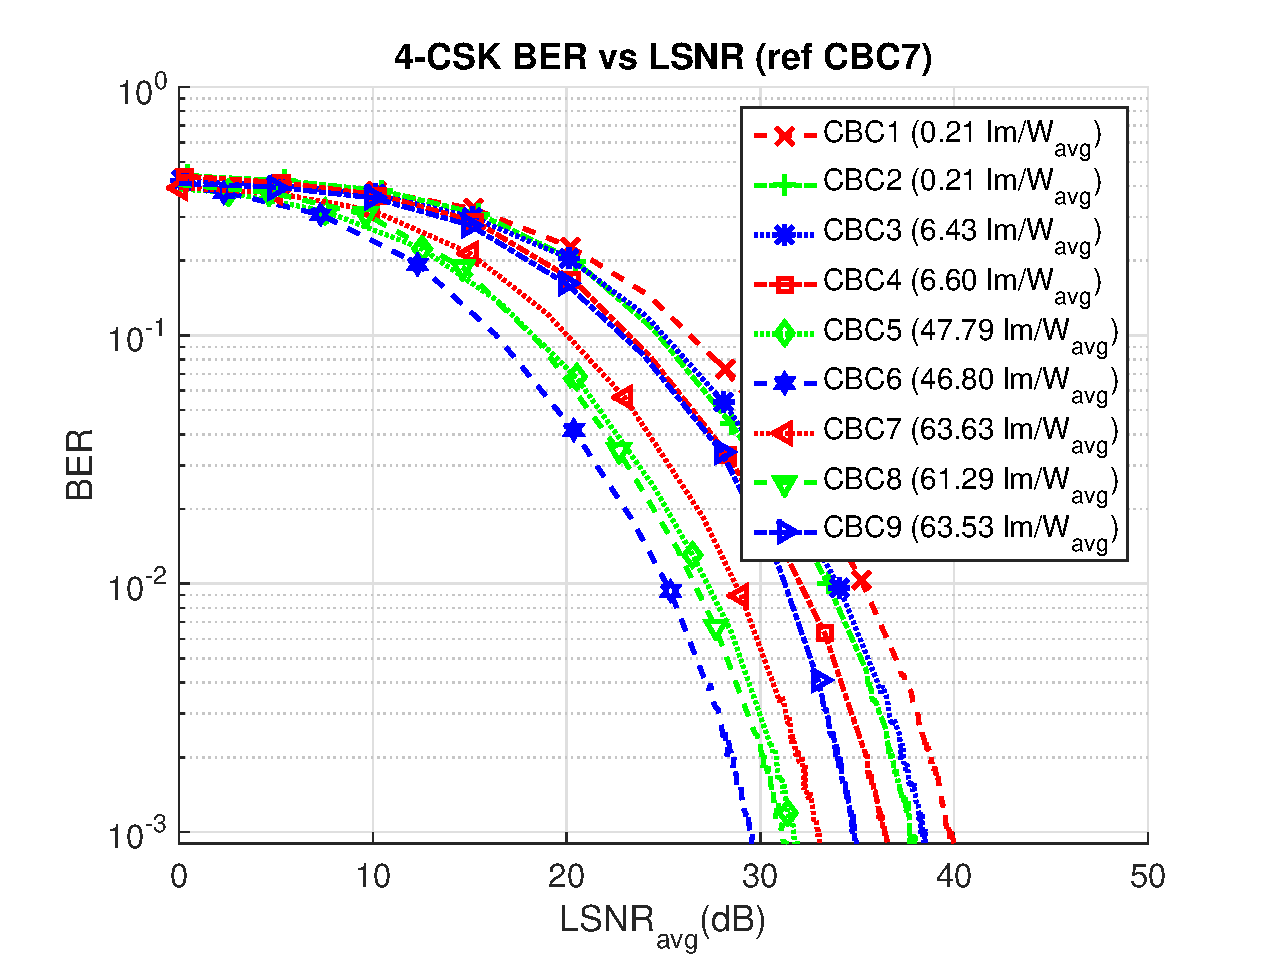
\includegraphics[trim={0.1in 0.0in 0.5in 0.1in}, clip=true, width=\textwidth]{M04_4-CSK_BERvsLSNR_NL.eps}
			\caption{4-CSK}
			\label{fig4LSNR}
		\end{subfigure}
		\hfill
		\begin{subfigure}{0.49\textwidth}
		\centering
			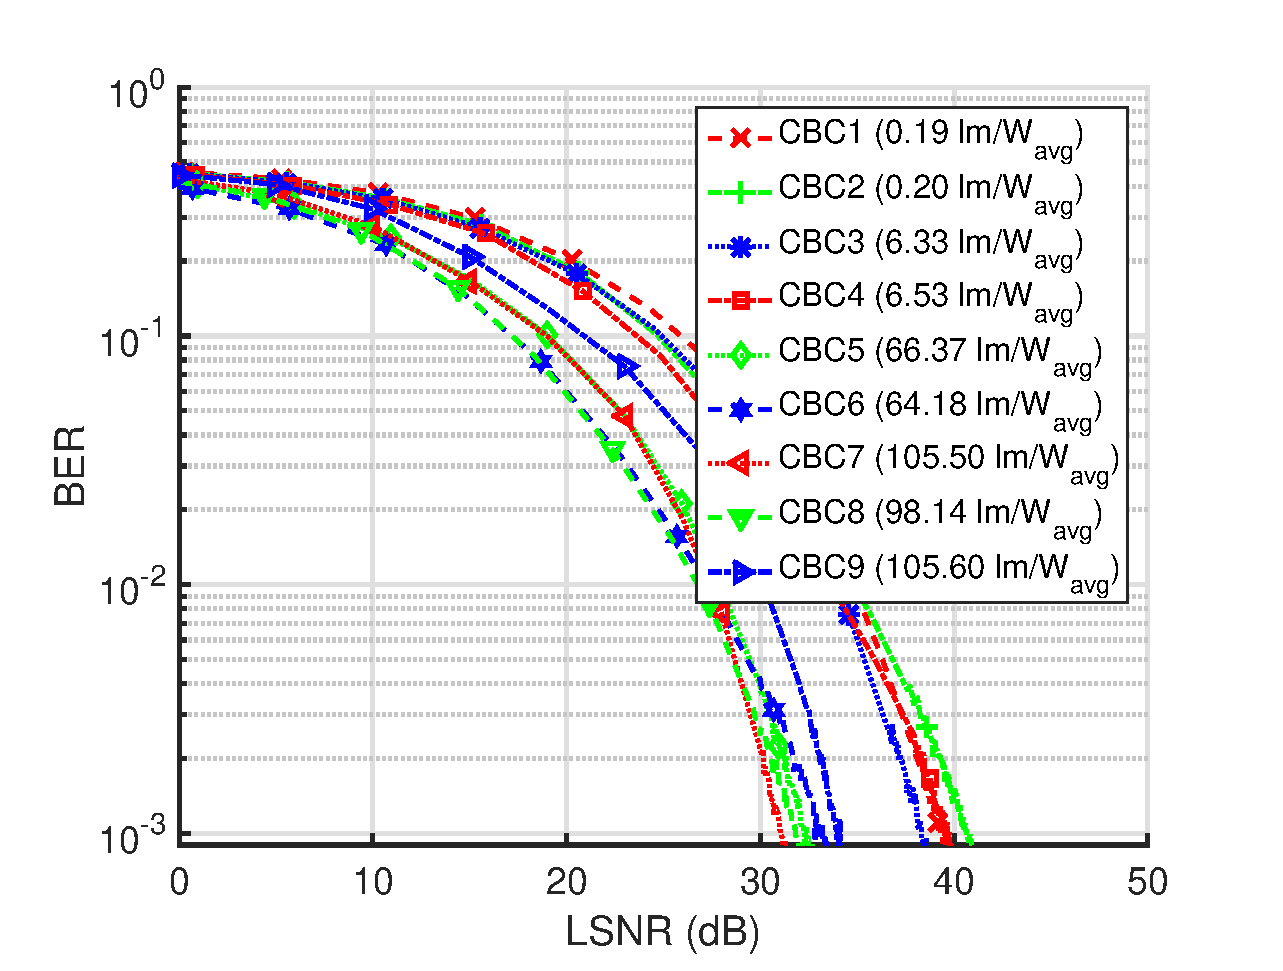
\includegraphics[trim={0.1in 0.0in 0.5in 0.1in}, clip=true, width=\textwidth]{M08_8-CSK_BERvsLSNR_NL.eps}
			\caption{8-CSK}
			\label{fig8LSNR}
		\end{subfigure}
		\vfill
		\begin{subfigure}{0.49\textwidth}
		\centering
			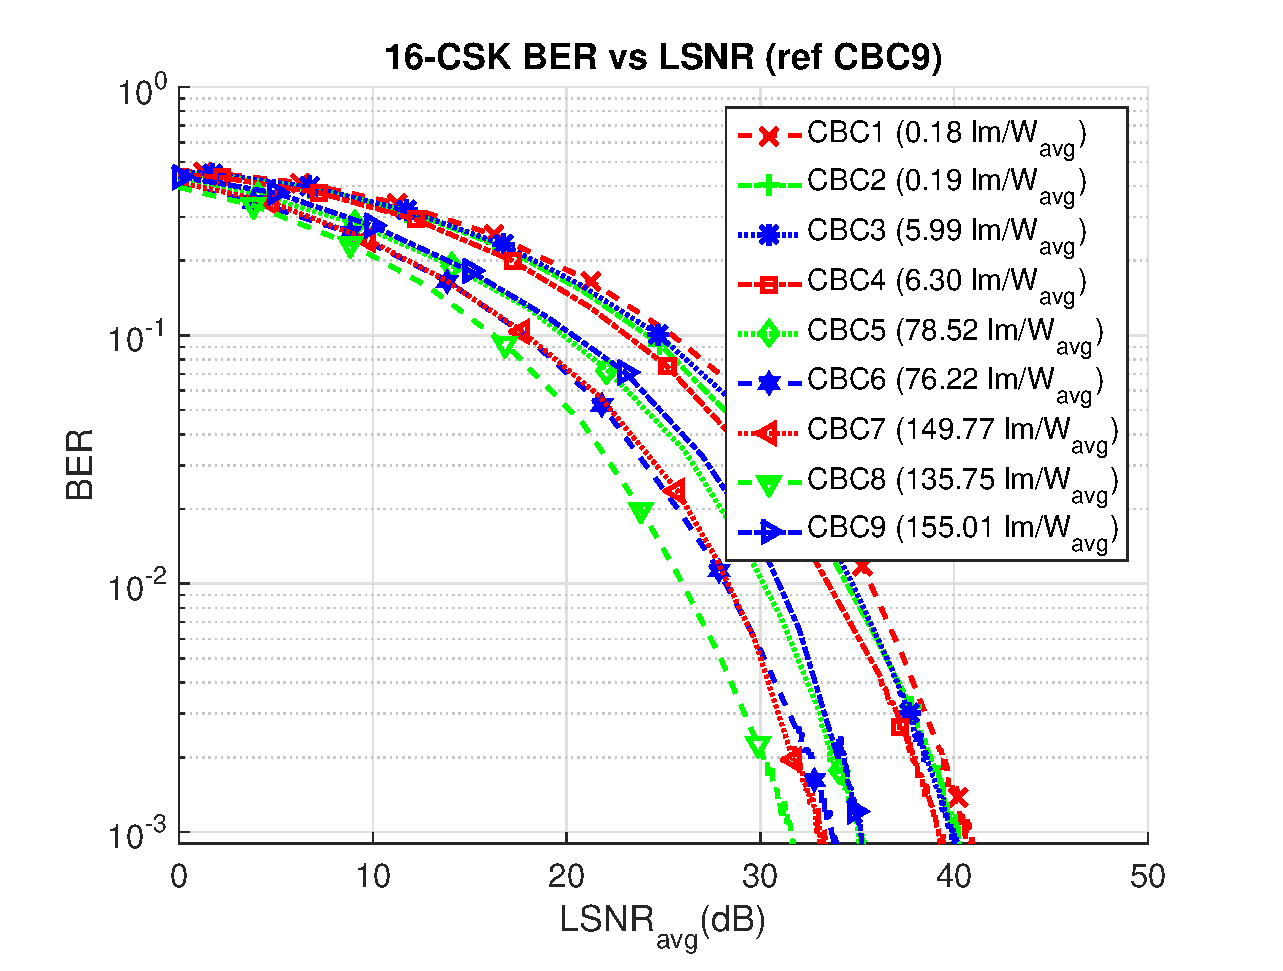
\includegraphics[trim={0.1in 0.0in 0.5in 0.1in}, clip=true, width=\textwidth]{M16_16-CSK_BERvsLSNR_NL.eps}
			\caption{16-CSK}
			\label{fig16LSNR}
		\end{subfigure}
	\caption{BER vs LSNR for all CBC}
	\label{figBERvsLSNR}
\end{figure}

In an indoor optical wireless system using lighting devices for wireless downlink access the luminaires need to simultaneously service illumination and optical wireless broadcast missions. Under this model, different colored PHY (example: different CBC$_{v}$) irradiate different amounts of radiant flux to achieve the same illumination intensity level. Thus, it is unfair to use SNR as a metric to compare performance of modulation schemes at same BER target using different colored PHY without first normalizing for illumination targets. Thus, in this section we introduce LSNR as a metric that takes into account the differences in radiant flux emitted by different PHY to achieve the same illumination intensity level. It should be noted that the LSNR metric is not specific to CSK, but instead can be used more generally to compare performance of any two optical modulation schemes that are operated at the same optical intensity levels.

Consider optical modulation scheme(s) which can be implemented with two different constellations C$_{\text{a}}$ or C$_{\text{b}}$. The fluxes emitted by the two constellations are scaled to achieve a target illumination intensity level. Let both constellations on average emit I lumens of luminous flux. Let the luminous efficacy for the two constellations be specified by $\eta_{\text{a}}$ and $\eta_{\text{b}}$ in lumens-per-watt respectively. Then the corresponding average radiant flux emitted by the two constellations is given by W$_{\text{a}}$ = I/$\eta_{\text{a}}$ and W$_{\text{b}}$  = I/$\eta_{\text{b}}$ watts respectively. Let us define a luminous ratio L$_{\text{ab}}\triangleq$ ($\eta_{\text{a}}/\eta_{\text{b}}$) $\equiv$ (W$_{\text{b}}$/W$_{\text{a}}$). Thus, for every 1 Watt of radiant flux emitted by C$_{\text{a}}$, C$_{\text{b}}$ must emit L$_{\text{ab}}$ Watt of radiant flux to achieve the same illumination intensity level. Under the model where the luminaires service illumination along with communication, it is fair to compare the performance of the two schemes at these relative radiant flux levels instead of at the absolute radiant flux levels. Thus we define the LSNR metric in Eq.\eqref{eqLSNR} as a means to compare performance of C$_{\text{b}}$ versus that of C$_{\text{a}}$ at same illumination levels. 

\begin{equation}
	% ^{ } is used with \vm{X} to help align subscript 'b' for both \vm{X} below.
	\text{LSNR}_{\text{ab}} \triangleq \frac{\text{L}^{2}_{\text{ab}}\text{Tr}\{\vm{H}\vm{X}^{ }_{\text{b}}\vm{X}^{*}_{\text{b}}\vm{H}^{*}\}}{\sigma^{2}_{n}} 
	\label{eqLSNR}
\end{equation}
where \vm{X}$_{\text{b}}$ is the average radiant flux emitted by C$_{\text{b}}$. Thus, after computing BER vs SNR for the scheme employing C$_{\text{a}}$, BER vs LSNR can be computed for scheme employing C$_{\text{b}}$ to compare its performance relative to that employing C$_{\text{a}}$ at the same illumination levels.

%%%%%%%%%%%%%%%%%%%%%  Illumination  %%%%%%%%%%%%%%%%%%%%%%%
\subsection{Performance under illumination constraints}\label{ssCSKLSNR}

\figurename{ }\ref{figBERvsLSNR} shows performance of the 9 CBCs under the non-linear model when normalized for illumination constraints. The efficacies of all CBC for different $M$ are specified in the legends. These values are used to normalize the performance of $M$-ary CSK for all CBC using CBC with highest efficacy as the reference for LSNR calculation. CBC$_{7}$, CBC$_{9}$ and CBC$_{9}$ are used as reference CBCs for $M$ = 4, 8 and 16 CSK respectively. The effect of this is to shift all curves (except the reference) from \figurename{ }\ref{figBERvsSNR_NL} towards left along the LSNR-axis depending on the L$_{\text{ab}}$ values in Eq.\eqref{eqLSNR}. It can be observed that given a target illumination intensity level and for target 10$^{-3}$ BER, CBC$_{6}$ performs the best for 4-CSK, CBC$_{7}$ and CBC$_{8}$ perform similar and better than others for 8-CSK and CBC$_{8}$ performs the best for 16-CSK. For CBC$_{1}$-CBC$_{4}$, due to their low luminous efficacy, one can use a much larger radiant flux to achieve target illumination levels and thus significantly improve their communication performance. However, this is achieved at the cost of poor energy efficiency. In contrast, CBC$_{7}$ and CBC$_{9}$ have relatively high luminous efficacy. This implies that these CBCs are restricted to emit a relatively lower radiant flux (and thus low signal powers) to achieve target illumination level thus affecting their communication performance. These results also highlight the necessary tradeoff between goals of energy efficient lighting and good communication performance; thus making a case for an optimization between the two divergent goals.

%%%%%%%%%%%%%%%%%%%%%%  Conclusion  %%%%%%%%%%%%%%%%%%%%%%%%
\section{Conclusion}\label{sCONC}

This article explores the performance of all CBCs as specified for $M$-ary CSK in the IEEE 802.15.7 standard. Under the linear system model, all CBCs perform relatively well and need SNR of at least 15 dB, 20 dB and 25 dB to
achieve target BER of $10^{-3}$ for $M$ = 4, 8 and 16 CSK respectively. The
non-linear system model is then considered due to the unique non-linear visual perception characteristics of human eye. It is shown that the
non-linearity of the CIE-CS causes the AWGN
introduced to the received signal to get skewed and no longer remain AWGN
when transformed to the chromaticity plane. Under the non-linear
system model, CBC$_{7}$ and CBC$_{8}$ perform relatively similar and are better that all other CBCs. A performance penalty
of at least 15 dB, 10 dB and 5 dB incurred for the practical non-linear model as compared to linear model for
$M$ = 4, 8 and 16 CSK respectively. A new LSNR metric is proposed
to compare performance of any two schemes (and not just CSK) using the visible
spectrum for wireless communication and lighting after normalizing signal powers to achieve a target illumination intensity level. Performance comparisons of $M$-ary CSK for all CBCs then reveal that CBC$_{6}$ performs the best for
4-CSK, CBC$_{7}$ and CBC$_{8}$ perform similar and better than others for 8-CSK and CBC$_{8}$ performs the best for 16-CSK. 

For IM/DD signaling scheme, the receiver output is always expected to be non-negative in absence of noise. For some O-OFDM systems, clipping negative receiver output has been shown to improve performance by eliminating some noise. On the contrary, for $M$-ary CSK, the performance in presence or absence of clipping the negative receiver output does not seem to differ significantly. This does not imply that noise in the negative receiver output is orthogonal to signal itself. The negative receiver output pushes the received symbol outside the color gamut on the CIE-CS. In the presence of relatively high SNR, the received symbol is still located closer to the expected constellation point thus does not introduce any additional errors.

Optimal performance of CSK can be seen as a tradeoff between the
illumination and communication missions. There is further scope to
optimize the $M$-ary CSK constellations under the practical non-linear
model by selecting optical sources centered at different wavelengths
than those considered in the standard. After characterizing skew for
AWGN along the chromaticity plane, constellation points can be
optimally positioned and optimal receiver architectures can be introduced to further improve the $M$-ary CSK performance.

%%%%%%%%%%%%%%%%%%%%  Acknowledgment  %%%%%%%%%%%%%%%%%%%%%%
\section*{Acknowledgment}
This work was supported by the Engineering Research Centers Program of the National Science Foundation under NSF Cooperative Agreement No. EEC-0812056.

\end{document}
